%%%%%%%%%%%%%%%%%%%%%%%%%%%%%%%%%%%%%%%%%%%%%%%%%%%%%%%%%%%%%%%%%%%%%%%%%%%%%%%%
%2345678901234567890123456789012345678901234567890123456789012345678901234567890
%        1         2         3         4         5         6         7         8
% DOCUMENT CLASS
\documentclass[oneside,12pt]{Classes/RoboticsLaTeX}

% USEFUL PACKAGES
% Commonly-used packages are included by default.
% Refer to section "Book - Useful packages" in the class file "Classes/RoboticsLaTeX.cls" for the complete list.
\usepackage{amsmath}
\usepackage{amsfonts}
\usepackage{algorithm}
\usepackage{algorithmic}
\usepackage{multirow}
\usepackage{colortbl}
\usepackage{color}
\usepackage[table]{xcolor}
\usepackage{epigraph}
\usepackage{graphicx}
%\usepackage{subfigure}
\usepackage{caption}
\usepackage{subcaption}
\usepackage{hyperref}
\usepackage{tabularx}
\usepackage{float}
\usepackage{longtable}
\usepackage[pdftex]{graphicx}
\usepackage{pdfpages}
\usepackage{hyperref}
\hypersetup{ colorlinks, citecolor=green, filecolor=black, linkcolor=blue, urlcolor=blue }
%\usepackage{tabularx}
\usepackage{pdflscape}
\usepackage{fourier} 
\usepackage{array}
\usepackage{makecell}
\usepackage[acronym,toc]{glossaries}
\usepackage{setspace}
\setstretch{1.5}
\newcommand{\angstrom}{\text{\normalfont\AA}}
\renewcommand\theadalign{bc}
\renewcommand\theadfont{\bfseries}
\renewcommand\theadgape{\Gape[4pt]}
\renewcommand\cellgape{\Gape[4pt]}
%\onehalfspacing
% SPECIAL COMMANDS
% correct bad hyphenation
\hyphenation{op-tical net-works semi-conduc-tor}
\hyphenation{par-ti-cu-lar mo-du-le ge-stu-re}
% INTERLINEA 1.5
%\renewcommand{\baselinestretch}{1.5}

%% ignore slightly overfull and underfull boxes
%\hbadness=10000
%\hfuzz=50pt
% declare commonly used operators
\DeclareMathOperator*{\argmax}{argmax}

% HEADER
\ifpdf
    \pdfinfo {/Title (MSc Thesis Draft (Working Title))
              /Creator (TeX)
              /Producer (pdfTeX)
              /Author (BGrant Cates)
              /CreationDate (D:20141024182500) %format D:YYYYMMDDhhmmss
              /ModDate (20141024182500)
              /Subject (Example of PhD Thesis with RoboticsLaTeX template)
              /Keywords (PhD, Thesis, Example, RoboticsLaTeX)}
    \pdfcatalog {/PageMode (/UseOutlines)
                 /OpenAction (fitbh) }
\fi

\title{\Large{MSc Thesis Draft (Working Title)}}

\ifpdf
  \author{Grant Cates
          }
  \collegeordept{Institute for Computational Physics}
  \university{University of Stuttgart}
  \crest{
\includegraphics[width=0.8\linewidth]{Figures/System/icplogo.png}}
\else
  \author{Grant Cates}
  \collegeordept{Institute for Computational Physics}
  \university{University of Stuttgart}
  \crest{
\includegraphics[width=30mm]{logo_unige}}
\fi
% nome relatore tesi 
\supervisor{Maria Fyta}

% DECLARATION
% Use the following command to change the declaration text:
%\renewcommand{\submittedtext}{INSERT NEW TEXT HERE}
\degree{Master of Science Physics}
\degreedate{\today}

%%%%%%%%%%%%%%%%%%%%%%%%%%%%%%%%%%%%%%%%%%%%%%%%%%%%%%%%%%%%%%%%%%%%%%%%%%%%%%%%
\makeglossaries
\loadglsentries{glossary}

\begin{document}

% A page with the abstract and running title and author etc may be
% required to be handed in separately. If this is not so, comment
% the following 3 lines:
% \begin{abstractseparate}
%   %%%%%%%%%%%%%%%%%%%%%%%%%%%%%%%%%%%%%%%%%%%%%%%%%%%%%%%%%%%%%%%%%%%%%%%%%%%%%%%%
%2345678901234567890123456789012345678901234567890123456789012345678901234567890
%        1         2         3         4         5         6         7         8
% THESIS ABSTRACT

% Use the following style if the abstract is long:
%\begin{abstractslong}
%\end{abstractslong}

\begin{abstracts}

The abstract goes here. The abstract should be self-contained and:
\begin{itemize}
    \item clearly state the problem dealt with by the thesis; \item give a synthetic description of the proposed solution;
    \item  highlight the sense in which the proposed solution enhances the state of the art.
\end{itemize}

\end{abstracts}

% \end{abstractseparate}
\begin{spacing}{1}
\maketitle
\end{spacing}

% add an empty page after title page
\newpage\null\thispagestyle{empty}\newpage

% set the number of sectioning levels that get number and appear in the contents
\setcounter{secnumdepth}{3}
\setcounter{tocdepth}{3}


\frontmatter
%%%%%%%%%%%%%%%%%%%%%%%%%%%%%%%%%%%%%%%%%%%%%%%%%%%%%%%%%%%%%%%%%%%%%%%%%%%%%%%%%
%2345678901234567890123456789012345678901234567890123456789012345678901234567890
%        1         2         3         4         5         6         7         8
% THESIS ACKNOWLEDGEMENTS

% Use the following style if the acknowledgements are long:
%\begin{acknowledgementslong}
%\end{acknowledgmentslong}

\begin{acknowledgements}


%“I don't know half of you half as well as I should like; and I like less than half of you half as well as you deserve.”
 %J.R.R. Tolkien, The Fellowship of the Ring 

Write here your acknowledgements...


\end{acknowledgements}

%%%%%%%%%%%%%%%%%%%%%%%%%%%%%%%%%%%%%%%%%%%%%%%%%%%%%%%%%%%%%%%%%%%%%%%%%%%%%%%%%
%2345678901234567890123456789012345678901234567890123456789012345678901234567890
%        1         2         3         4         5         6         7         8
% THESIS DEDICATION

\begin{dedication}

% quote
Thesis dedication goes here...
\end{dedication}

% ----------------------------------------------------------------------

%%% Local Variables: 
%%% mode: latex
%%% TeX-master: "../thesis"
%%% End: 

%%%%%%%%%%%%%%%%%%%%%%%%%%%%%%%%%%%%%%%%%%%%%%%%%%%%%%%%%%%%%%%%%%%%%%%%%%%%%%%%%
%2345678901234567890123456789012345678901234567890123456789012345678901234567890
%        1         2         3         4         5         6         7         8
% THESIS ABSTRACT

% Use the following style if the abstract is long:
%\begin{abstractslong}
%\end{abstractslong}

\begin{abstracts}

The abstract goes here. The abstract should be self-contained and:
\begin{itemize}
    \item clearly state the problem dealt with by the thesis; \item give a synthetic description of the proposed solution;
    \item  highlight the sense in which the proposed solution enhances the state of the art.
\end{itemize}

\end{abstracts}


\tableofcontents
\listoffigures
\listoftables
\printglossary[title=List of Acronyms,type=\acronymtype]
%\printglossary  % Print the nomenclature (WAY TOO COMPLEX FOR ME NOW!)
%\addcontentsline{toc}{chapter}{Nomenclature}

\mainmatter
%%%%%%%%%%%%%%%%%%%%%%%%%%%%%%%%%%%%%%%%%%%%%%%%%%%%%%%%%%%%%%%%%%%%%%%%%%%%%%%%
%2345678901234567890123456789012345678901234567890123456789012345678901234567890
%        1         2         3         4         5         6         7         8
% THESIS INTRODUCTION

\chapter{Introduction}
\label{chap:introduction}
\ifpdf
    \graphicspath{{Introduction/Figures/PNG/}{Introduction/Figures/PDF/}{Introduction/Figures/}}
\else
    \graphicspath{{Introduction/Figures/EPS/}{Introduction/Figures/}}
\fi

Water is one of the most ubiquitous, and universally experienced, substances on this planet. It is rather counter-intuitive, then, how much remains to be understood about water. The situation is even more precarious when more exotic forms of water are concerned, for instance water at extremely high pressures or within nanoscale confinement. The latter of these two is the primary focus of this study. Specifically, how does the confinement of single water molecules in the naturally occurring nanocages of the beryl crystal affect its structural and electronic properties? 



\section{Context of and Motivations for Study}
\label{motivations}

Confined water has been the subject of numerous studies, and is believed to be broadly applicable, including in mineralogy, geology, climatology, meteorology and cosmology; but the area of greatest potential impact is in biology [\textbf{list of citations}]. Biological systems often create naturally occurring channels wherein individual water molecules traverse the system or interfaces where single molecules are participating in hydrophilic/hydrophobic interactions, transcription and replication processes. If these biological processes are to ever be fully understood, the effects of confinement need to be fully understood. Unfortunately, attempting to study confined water in biological is extremely difficult, for any interpretation of the experimental results is obfuscated by the systems’ complexity. Studies of simpler systems, then, are needed to gain insight into the fundamental mechanisms behind these biological processes.  

Nature has provided an ideal “scaffolding” with which to perform such a study, namely with a family of crystals of which beryl is a member. Like all crystals, the periodic nature of these structures provides the idyllic, simple geometry that biological systems often lack. Additionally, beryl crystals contain naturally occurring cavities, or nanocages, with dimensions perfectly suited for trapping single water molecules. When beryl crystals are grown in water environments, single water molecules are trapped within said nanocages. Moreover, these nanocages are spaced at such a distance that the hydrogen bonds that dominate the bulk characteristics of water are interrupted, and the dipole interactions are able to govern.
 
Some explorations of this system have already been conducted, both theoretically and experimentally, which provide the foundation for this study. From optical spectroscopy experiments, two different types of confined water have been identified [\textbf{nature paper}], as well as the different vibrational modes accessible to said water molecules [\textbf{vibrational spectra paper}]. The system has also been probed theoretically, where it is believed to be a good candidate for a quantum electric dipole system [\textbf{qed paper}]. 

These studies have provided a macroscopic-esque view of the system, but want for a low-level investigation of the dipole-dipole dynamics still exists. Due to the time- and length scales of this system, such investigations should be carried out computationally.

\section{Objectives and Contributions}
\label{objectives}

The primary objective of this project is to provide foundational knowledge so that larger computational studies can be performed. To that end, assumptions about the coupling between the crystal framework and the extra-framework water molecules need to be tested, the geometry of the water molecules needs to be determined with respect to fill factor and relative position to other water molecules and the framework, a potential energy map for the high-symmetry point needs to be calculated over the same fill and relative position parameter space, and the molecular dipole needs to be determined in all of these cases as well. Finally, the contributions of the crystal framework and of the water-water subsystems need to be disentangled.

As previously mentioned, beryl is a single example of a class of crystals in which such a study can be performed. As such, the "path of least computational resources" will be identified, so that future studies of these other crystals can be performed in a systematic, cost-effective way. 

\section{Overview of the Thesis}
\label{overview}

The remainder of this thesis is broken down into five chapters. First, the necessary background information is presented, including theory, system overview, and details of the calculations. The following three chapters represent the bulk of this work and present the structural optimization, potential map calculations, and partial charge analysis. Each chapter is further subdivided into separate experiments, wherein the motivation, procedure, results, and analyses are presented. At the end of each chapter, a brief summary of all of the results is provided as well as an outlook for future work. The concluding chapter provides a high-level summary of the work in its entirety as well as a general outlook for the computational investigation of this system.
\chapter{Background Information}   

Here, necessary background information is presented. To begin, a cursory overview of the necessary theory is provided. Then the system under investigation is introduced. Finally, details relating to software packages and default parameters are listed.
    
    \section{Theory}
    
    In the following chapter, the necessary theory to understand this work and its analysis is presented. The explanations below are not meant to be exhaustive, rather the minimal set of information needed for comprehension. For readers seeking more information, additional sources are cited.
    
    To start, a high-level overview of Density Functional Theory is presented, followed by a quantum mechanical technique called Wannierization. Finally, an introduction to force fields is provided to better elucidate the goals of this research.
    
    Certain assumptions are made regarding the reader's background knowledge. A certain familiarity with quantum mechanics and solid state physics is assumed. Specifically, it is assumed the reader is familiar with enough quantum mechanics to understand the quantum description of the hydrogen atom and the concepts of the unit cell, reciprocal space, and Bloch functions. 
    
    \subsection{Density Functional Theory}
    
    Density Functional Theory (DFT) is a quantum mechanical technique used to the solve interacting many-body problems and attain an approximation for the groundstate wavefunction of a system [\textbf{bird's eye view of dft paper}]. 
    
    To appreciate what DFT has to offer from a high-level, first consider a system of ions and electrons, totally $N$ bodies. Solving any equation for such a system is a $3N$ dimensional problem. This dimensionality can be (drastically) reduced (in the case of large $N$) if one considers rather the ion and electron densities. Since the Born-Oppenheimer (BO) approximation is typically invoked\textemdash that is, the ionic and electronic systems can be decoupled\textemdash this reduces the problem to solving for a 3-dimensional wavefunction. Still, such a solution is not easily come by, and additional machinery is needed.
    
        \subsubsection{Hohenberg-Kohn Theorems} 
        
        The theoretical underpinning for DFT comes from the Hohenberg-Kohn (HK) theorems. They are as follows: (HK-1) There exists a one-to-one mapping between the groundstate electron density $n(\Vec{r})$ and the groundstate wavefunction $\psi (\Vec{r})$ for a non-degenerate groundstate, and (HK-2) The groundstate density $n_0(\Vec{r)}$ minimizes the total energy. [\textbf{HK 1964 paper}]
        
        Taken together, the HK theorems provide a road map for solving the interacting many-body problem. Rather than treating each interacting body explicitly, the electron \textit{density} of the groundstate is sought. Once that is determined, a simple mapping is applied to attain the groundstate wavefunction $\psi_0$.
        
        Note, the first HK theorem (HK-1) is in essence an existence theorem, not a construction theorem. Rather than identify the specific mapping between groundstate density and groundstate wavefunction, it proves that such a mapping exists. To construct such a mapping, one uses the Kohn-Sham equation.
        
        \subsubsection{Kohn-Sham Equation} 
        
        The Kohn-Sham (KS) equation is a single-particle, Schr{\"o}dinger-like equation for a fictitious system of non-interacting particles that produces the same groundstate density as the interacting many-body system. It takes the form
        
        \begin{equation}
            \label{eq:ks}
            \left[-\frac{\hbar^2}{2 m}\nabla^2 + V_\text{eff}(\Vec{r}) \right]\phi_i(\Vec{r}) = \varepsilon_i \phi_i(\Vec{r}),
        \end{equation}
        
        \noindent for reduced Planck constant $\hbar$, electron mass $m$, gradient operator $\nabla$, an effective potential $V_\text{eff}$, and fictitious KS-orbitals $\phi_i$ with corresponding KS-energy $\varepsilon_i$. (Note, again the BO approximation is invoked here.) The density of the original $N$-body problems is related to the fictitious KS-orbitals by
        
        \begin{equation}
            n(\Vec{r}) = \sum\limits_{i=1}^N |\phi_i(\Vec{r}) |^2
        \end{equation}
        
        The total energy for the KS-system is given by
        
        \begin{equation}
        \label{eq:func1}
            E[n] = T[n] + E_\text{ext}[n] + E_\text{H}[n] + E_\text{xc}[n],
        \end{equation}
        
        \noindent with KS-kinetic energy
        
        \begin{equation}
        \label{eq:func2}
            T[n] = \sum\limits_{i=1}^N \int \phi_i^*(\Vec{r})\left(-\frac{\hbar^2}{2m}\nabla^2 \right)\phi_i(\Vec{r})d\Vec{r},
        \end{equation}
        
        \noindent external energy using the system-specific external potential $\nu_\text{ext}$
        
        \begin{equation}
            E_\text{ext}[n] = \int \nu_\text{ext}(\Vec{r}) n(\Vec{r})d\Vec{r},
        \end{equation}
        
        \noindent Hartree/Coulomb correlation 
        
        \begin{equation}
        \label{eq:func3}
            E_\text{H}[n] = \frac{e^2}{2}\int\int \frac{n(\Vec{r})n(\Vec{r'})}{|\Vec{r} - \Vec{r'}|}d\Vec{r}d\Vec{r'}, 
        \end{equation}
        
        \noindent and exchange-correlation (xc) energy $E_\text{xc}$ which is discussed in detail below. 
        
        (As a nomenclature note, eqs. (\ref{eq:func1}-\ref{eq:func3}) are functionals as denoted by the use of $[\text{ }]$. Put simply a functional is a function that takes other functions, such as the density $n(\Vec{r})$, as inputs.)
        
        The latter three terms in (\ref{eq:func1}) are related to what is often called the KS-effective potential
        
        \begin{equation}
            V_\text{eff}(\Vec{r}) = \nu_\text{ext}(\Vec{r}) + \frac{e^2}{2}\int \frac{n(\Vec{r'})}{|\Vec{r}- \Vec{r'}|} d\Vec{r'} + \nu_\text{xc}(\Vec{r}),
        \end{equation}
        
        \noindent with the xc-potential $\nu_\text{xc}$ defined as
        
        \begin{equation}
            \nu_\text{xc}(\vec(\vec{r})) = \frac{\partial E_{xc}[n(\vec{r})]}{\partial n(\vec{r})},
        \end{equation}
        
        \noindent which encompasses all other many-body interactions and is the only component that is not known exactly, and approximations must be made. More on that below.
        
        \subsubsection{Exchange-Correlation Functional}
        
        Broadly stated, exchange-correlation refers to all of the interactions between the many-bodies with corresponding xc-energy $E_\text{xc}$. In the case of fermions, the exchange refers to the well-known Pauli exclusion principle, and the correlation refers to all other correlations with the exception of the Hartree/Coulomb correlation, for which eq. (\ref{eq:func3}) already accounts. The corresponding energy is thus
        
        \begin{equation}
            \label{eq:xc_energy}
            E_\text{xc}[n(\Vec{r})]= \int \left\{ \varepsilon_\text{x}[n(\Vec{r})] + \varepsilon_\text{c}[n(\Vec{r})]\right\} n(\vec{r})d\vec{r},
        \end{equation}
        
        \noindent with exchange potential $\varepsilon_\text{x}$ and correlation potential $\varepsilon_\text{c}$.
        
        As the use of phrases such as "all other correlations" may suggests, eq. (\ref{eq:xc_energy}) is not known exactly and is where errors are introduced to DFT. Collectively, these potentials are known as the xc-functional $\varepsilon_\text{xc} = \varepsilon_\text{x} + \varepsilon_\text{c}$ and approximations must be used.
        
        \paragraph{Local-Density Approximation} One of the basic approximations is the Local Density Approximation (LDA), which depends solely upon the electron density at a given point
        
        \begin{equation}
            \varepsilon_\text{xc}[n(\vec(r))] \approx \varepsilon_\text{xc}^\text{LDA}[n(\vec(r))].
        \end{equation}
        
        \noindent Here, $\varepsilon_\text{xc}^\text{LDA}$ is the xc-functional for a homogeneous electron gas (HEG) with density $n$. An analytic form of the exchange component is known, but the correlation component is only known exactly in limiting cases [\textbf{bird's eye view}]. 
        
        \paragraph{Generalized Gradient Approximation} Implicit in the description above, the LDA assumes that the density does not vary, or put differently, the gradient of the density vanishes. While this is true in the case of the HEG, it is not generally so, and this discrepancy often manifests itself by (under-) over-estimating the (exchange) correlation energy [\textbf{10.1063/1.4869598}]. To combat this, the LDA functional is expanded to include the gradient of the density 
        
        \begin{equation}
        \label{eq:gga}
            \varepsilon_\text{xc}[n(\vec(r))] \approx \varepsilon_\text{xc}^\text{GGA}[n(\vec(r)),\nabla n(\vec(r))].
        \end{equation}
        
        \noindent Conceptually, this can be thought of as the first correction to the Taylor expansion of the density at point $\vec{r}$. While one could in theory use as many terms in this expansion as desired, this work uses functionals of the form (\ref{eq:gga}) throughout.
        
        \subsubsection{Variational Principle}
        
        Before putting all of the above theoretical pieces together, one more piece is needed to form a high-level understanding of DFT\textemdash the variational principle. From calculus of variations, it is known that any physical quantity that depends on a set of equations can be optimized by an element in that set. The generalized methods by which this function is obtained is referred to as the variational principle [\textbf{ISBN 0-8020-1743-6}]. Note, an implicit assumption in the above statement is that the quantity, or observable, being measured is bound on at least one end.
        
        To unpack this definition contextually, consider the energy $E$ of some quantum mechanical system, which is a functional of the wavefunction $\psi$
        
        \begin{equation}
        \label{eq:en_var}
            E \rightarrow E[\psi(\vec{r})].
        \end{equation}
        
        \noindent Knowing that the system has some groundstate energy $E_0$ described by some groundstate wavefunction $\psi_0$, the energy value in (\ref{eq:en_var}) is strictly greater than or equal to the true groundstate energy. That is,
        
        \begin{equation}
            \label{eq:varprinc}
            E_0 = E[\psi_0(\vec{r})] \le E[\psi(\Vec{r})].
        \end{equation}
        
        Equation (\ref{eq:varprinc}), coupled with the HK theorems, hints at a protocol for approximating the groundstate energy, and therefore wavefunction. This protocol is summarized below.
        
        \subsubsection{Algorithm Summary}
        
        Before presenting the algorithm, consider what is known:
        
        \begin{itemize}
            \item There exists a one-to-one mapping between the groundstate wavefunction $\psi_0$ and the groundstate electron density $n_0(\Vec{r})$, and $n_0(\Vec{r})$ minimizes the total energy (e.g. gives the groundstate energy $E_0$). (HK 1-2)
            \item The groundstate density $n_\text{KS}(\Vec{r})$ of the fictitious KS system is the same as the groundstate density $n_0(\Vec{r})$ of the quantum system. 
            \item Any trial wavefunction $\psi(\Vec{r})$ corresponds to energy greater than or equal to the groundstate energy.
        \end{itemize}
        
        \noindent Leveraging the above information, the following self-consistent algorithm is implemented in DFT.
        
        \begin{enumerate}
            \item An initial guess of the density $n_k(\Vec{r})$ is made.
            \item The effective potential $V[n_k(\vec{r})]$ is evaluated.
            \item The KS equation (\ref{eq:ks}) is solved.
            \item The new density is calculated $n_{k+1}(\Vec{r}) = \sum\limits_{i=1}^N |\phi_i(\vec{r})|^2$.
            \item The following statement is evaluated as True of False for some tolerance $\delta$:
        \end{enumerate}
        
        \begin{equation}
        \label{eq:self_con}
            |n_{k}(\vec{r}) - n_{k+1}(\vec{r})| \le \delta.
        \end{equation}
        
        \noindent In the event that (\ref{eq:self_con}) is not true, steps 1-5 are repeated using $n_{k+1}(\Vec{r})$ as the trial density, and this process continues until self-consistency is achieved. Once achieved, the wavefunction associated with the self-consistent density is determined to be the groundstate.
        
        While the exact subroutines that accomplish steps 1-5 vary by implementation, they are not necessary for the understanding, and are beyond the scope, of this work. Even with these black boxes, though, a high-level appreciation for the DFT approach is possible.
    
    \subsection{Wannierization}
    
    Wannierization describes a change of basis transformation from one basis set to Wannier functions, which can serve as a basis set for periodic solids. Consider, for instance, the commonly used basis set comprised of Bloch orbitals
    
    \begin{equation}
    \label{eq:wan_1}
        \Psi_{n,\vec{k}}(\Vec{r}) = e^{i\Vec{k}\cdot\Vec{r}} e^{i\varphi_n(\vec{k})} u_n(\vec{r}), 
    \end{equation}
    
    \noindent for wavenumber $\vec{k}$, arbitrary phase factor $e^{i\varphi_n(\vec{k})}$, and some function $u_n(\vec{r})$ with the same periodicity as the structure. The Wannier function (WF) is found by applying a unitary transformation, yielding
    
    \begin{equation}
    \label{eq:wan_2}
        w_{n,\vec{R}}(\Vec{r}) = \frac{V}{(2\pi)^3} \sum\limits_{\Vec{k}}  \Psi_{n,\vec{k}}(\Vec{r}) e^{-i\Vec{k}\cdot\Vec{R}} e^{i\varphi_n(\vec{k})},
    \end{equation}
    
    \noindent for specific lattice site $\vec{R}$. Note, the similarities between (\ref{eq:wan_1}) and (\ref{eq:wan_2}) and that of a Fourier transformation. In both, a mapping between real- and reciprocal space occurs. In fact, in the case of Wannierization, the Bloch orbitals, which are localized in reciprocal space, are transformed into Wannier functions, which are localized in real space.
    
    It is worth noting that the WF (\ref{eq:wan_2}) is not unique due to the arbitrary phase factor $e^{i\varphi_n(\vec{k})}$, but this arbitrariness is exploited to choose a WF that minimizes the \textit{spread} $\Omega$, which is defined by
    
    \begin{equation}
        \Omega \equiv \sum\limits_n \left[ \langle r^2 \rangle_n - \langle r \rangle^2_n \right]
    \end{equation}
    
    \noindent Such WFs, known as maximally localized wannier functions (MLWFs) are extremely useful to understand the system chemically and can be thought of as the conceptual analog to molecular orbitals in periodic solids [\textbf{wannier review}].
    
    
    There exist many reasons for doing such a transformation (see [\textbf{wannier review}] for extensive review of theory and applications), but the impetus for this study lies in partial change analysis. It turns out the the centers of the MLWFs can be thought of as the classical location for the point charge, and the sum of all of the centers is related to the polarization [\textbf{wannier review}]. More details on how this technique is utilized are given in the Chapter \ref{ch:part_char}.
    
    Again, the actual subroutines implemented to calculated the MLWFs and their corresponding centers are treated as a black box for the purposes of this study.
    
    \subsection{Force Fields}
    
    There are many reasons why one would want to avoid using the DFT techniques described above when computationally investigating a system. For starters, DFT calculations generally require significant computational resources, to the point that running certain calculations in this work require access to some type of cluster. There are benefits to this higher cost though, specifically the electronic subsystem's degrees of freedom are, in fact, free. When trying to calculate the effect on a molecule's dipole in the presence of other atoms, for example, it is necessary that the electronic subsystem can interact.
    
    What if, though, the obversable of interest in not dependent explicitly on the electronic subsystem\textemdash say, the dynamics of $N$ molecules in a box of volume $V$. Here, fluctuations in the electronic subsystem are assumed negligible for purposes of interaction calculations, and it is reasonable to assign point charges to the atoms, effectively freezing the electronic degrees of freedom. 
    
    Assigning such a point charge is an example of a parameter and dramatically decreases computational cost, because the expensive DFT procedures can be skipped. But it immediately begs the question: how much charge do you assign to each atom? The process by which this question is answered is known as parameterization.
    
        \subsubsection{Parameterization}
        
        In general, parameterization is the process by which the total energy $E_T$ of a system is decomposed into independent contributions, namely bonded and non-bonded energy
        
        \begin{equation}
            E_T = E_B + E_N.
        \end{equation}
        
        \noindent The bonded and non-bonded energies can each be further decomposed (into bond, angle, and dihedral energies; and van der Waals and Coulomb energies respectively), wherein each one of these energies corresponds to a certain interaction.
        
        \begin{figure}
            \centering
            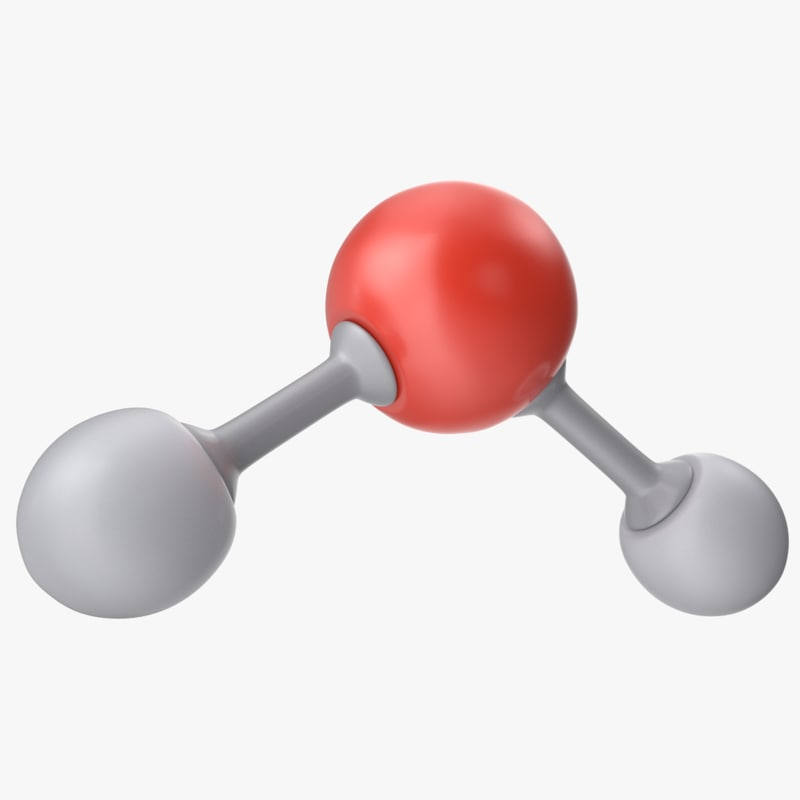
\includegraphics[width=0.4\linewidth]{Figures/System/water-molecule.jpg}
            \caption{Depiction of a water molecules with one oxygen atom (red) and two hydrogen atoms (silver). The two covalent bonds are indicated by a white bar. [\textbf{turbosquid.com}]}
            \label{fig:water_molecule}
        \end{figure}
        
    
            \paragraph{Ex: H$_2$O Molecule Force Field}
    
            To unpack this rather convoluted general definition, consider the case of a water molecule as shown in Fig. \ref{fig:water_molecule}. Between the oxygen atom (red) and each of the hydrogen atoms (silver), there exists a bond potential, given by
            
            \begin{equation}
            \label{eq:bond_param}
                E_\text{bond} = k_b(|\vec{r}|-|\vec{r_0}|),
            \end{equation}
            
            \noindent for separation vector $\vec{r}$, equilibrium separation vector $\vec{r_0}$, and bond parameter $k_b$. In order to use (\ref{eq:bond_param}), values must be provided for the bond parameter and the equilibrium separation vector.
            
            Similarly, one can imagine an angle potential corresponding to the expansion and contraction of the OHO angle $\theta$
            
            \begin{equation}
                E_\text{ang} = k_a(\theta - \theta_0),
            \end{equation}
            
            \noindent for angle parameter $k_a$ and equilibrium OHO angle $\theta_0$. Again, both of these require a numeric value to be of any use. Additionally, each atomic species has a partial charge assigned to it, such that the total charge vanishes.

            
            \paragraph{Tuning Parameter Value} There are numerous options for determining the parameter values, but the general procedure is the same. Some initial guess is made, typically in reference to a value from experiment or more-accurate quantum calculation, and an experiment is performed to measure an observable. For instance, the in the case of the water molecule, and box of water may be simulated at ambient conditions and the density of water molecules is measured. This measured density can be compared to the reference value, and if the results are not satisfactory, the parameters are adjusted slightly and the experiment is repeated. This process continues until the force field reproduces the correct density, at least in a satisfactory manner.

    \section{System Overview}
    
    In the following, the system under investigation is briefly introduced. First, the framework crystal beryl is presented with relevant structural data followed by the extra-framework water. Throughout this work, more specific system details will be highlighted as necessary. This section is mainly concerned with introducing the reader to the system.
    
        \subsection{Beryl Framework}
        
        \begin{figure}
            \centering
            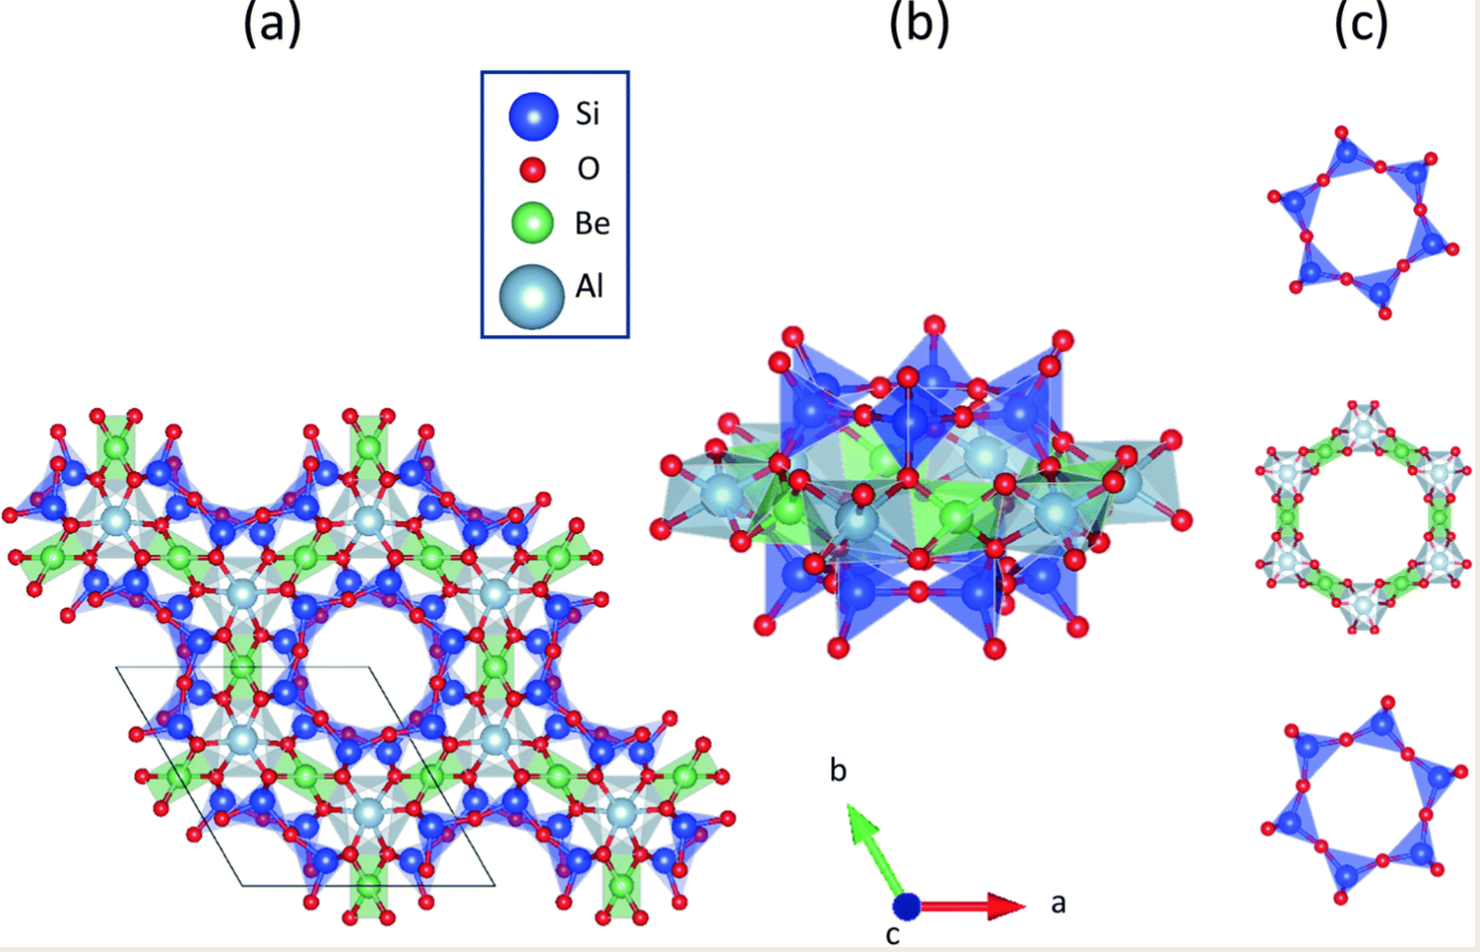
\includegraphics[width=0.9\linewidth]{Figures/System/beryl_structure.png}
            \caption{Different representation of the beryl structure: (a) Top-down view of a beryl supercell, (b) askew view of single nanocage, (c) top-down view of nanocage components. See text for details. [\textbf{10.1039/c7cp06472a}]}
            \label{fig:beryl_structure}
        \end{figure}
        
        Beryl (Be$_3$Al$_2$Si$_6$O$_{18}$) is a hexagonal crystal composed on beryllium, silicon, aluminum, and oxygen atoms. The structure (shown in Fig. \ref{fig:beryl_structure}) can be decomposed into two components: a beryllium-aluminum octohedral backbone and silicon-oxygen tetrahedral rings. 
        
        When the unit cell (depicted in grey) is repeated, hollow channels formed when view along the $c$-axis (Fig. \ref{fig:beryl_structure}a). When viewed from the side, it is clear that these silicon-oxygen rings forms bottlenecks along the channel effectively creating a periodic array of nanocages (Fig. \ref{fig:beryl_structure}b), with each cage made up of two silicon-oxygen rings and one beryllium-aluminum ring (Fig. \ref{fig:beryl_structure}c).
        
        \begin{figure}
            \centering
            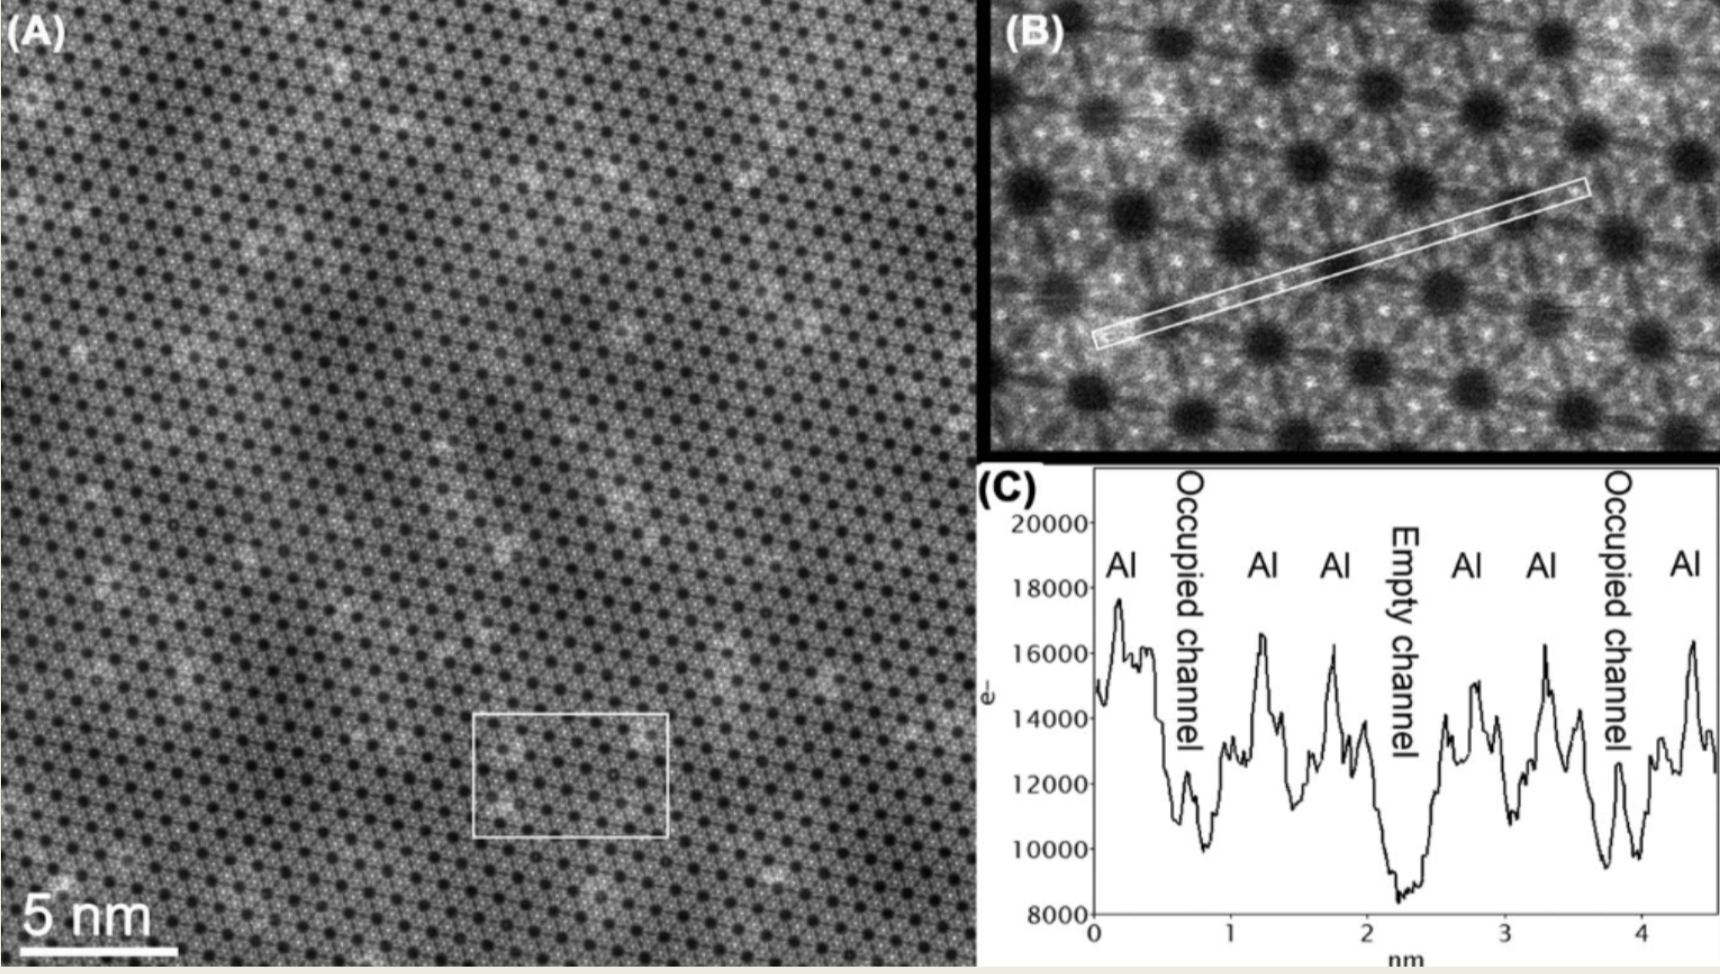
\includegraphics[width=0.9\linewidth]{Figures/System/beryl_tem.png}
            \caption{(A) Dark field TEM image of a sample of beryl variety; (B) enlarged region of TEM image, in which extra-framework species are visible; (C) line-cut intensity along path highlighted by box in (B) showing unambiguously the presence of extra-framework species.}
            \label{fig:beryl_tem}
        \end{figure}
        
        A dark-field tunneling electron microscope (TEM) image viewed down the $c$-axis is shown in Fig. \ref{fig:beryl_tem}. The hexagonal structure and channels are clearly visible in Fig. \ref{fig:beryl_tem}A, and when a smaller region is examined in detail (Fig. \ref{fig:beryl_tem}B) some of the channels appear to be occupied. By looking at an intensity line cut along the path highlighted in Fig. \ref{fig:beryl_tem}B, the occupation of the first and third channels in unambiguous. 
        
        Identification of the extra-framework species is not immediately clear from Fig. \ref{fig:beryl_tem}, but further studies have shown that these species can be cations or, as is of interest for this study, single water molecules [\textbf{nature paper}].
        
        \subsection{Extra-Framework Water}
        
        \begin{figure}
            \centering
            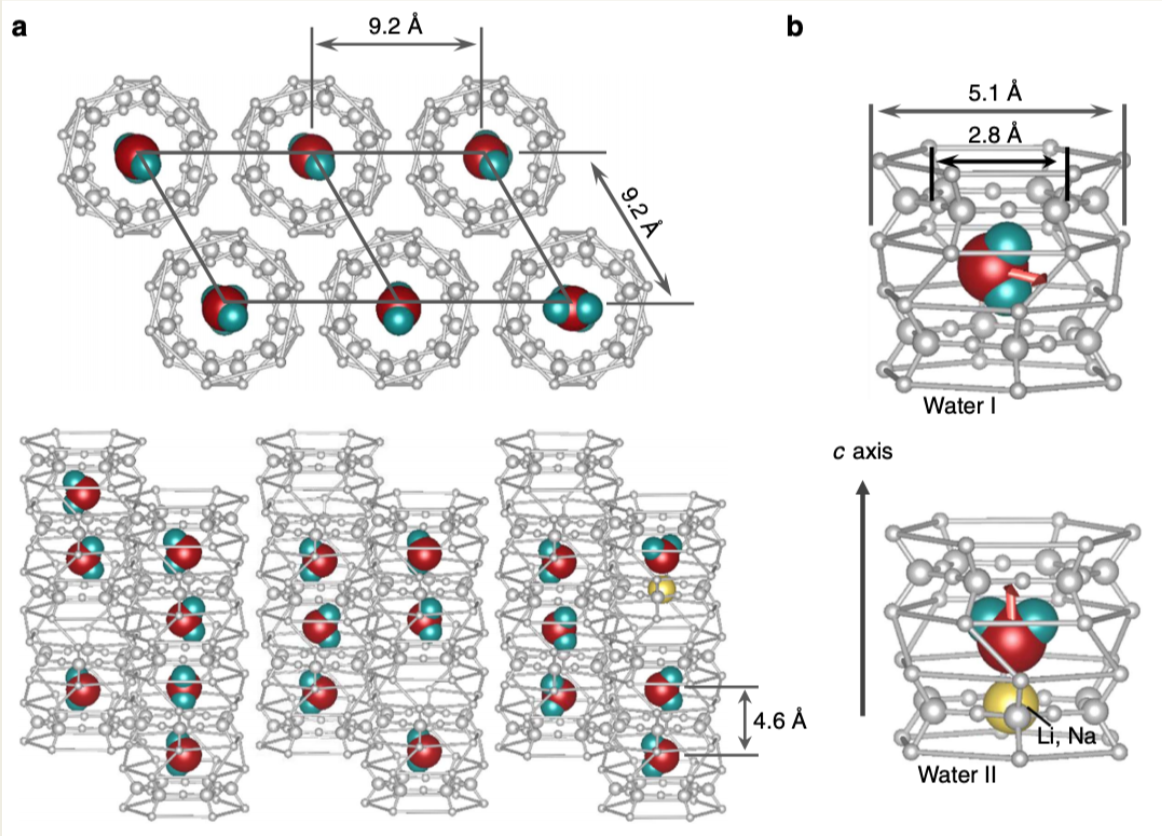
\includegraphics[width=0.9\linewidth]{Figures/System/beryl_water.png}
            \caption{Diagrams showing water molecules confined in beryl nanocages and relevant geometries. The backbone is omitted for visual clarity. (A) Top-down and side view of six channels of cages, (B) Individual cages containing types I, II water molecules. [\textbf{nature paper}]}
            \label{fig:beryl_water}
        \end{figure}
        
        Beryl crystal are grown hydrothermally, and as part of that process, water molecules become trapped in the nanocages, as shown in Fig. \ref{fig:beryl_water}. Within the $ab$-plane, the water molecules are separated by a distance of 9.2 $\angstrom$ and 4.8 $\angstrom$ along the $c$-axis. This partitioning interrupts the hydrogen bond network typically found in water systems. As a result, the water molecules interact solely via the dipole-dipole interaction. 
        
        \paragraph{Water Types} Depending on the existence of additional foreign atoms, there exists two types of confined water. The first, type I, exists in the absence of any other foreign atom with the dipole moment in the $ab$-plane (Fig. \ref{fig:beryl_water}b, top). Relevant degrees of freedom include in-plane translation and librations (i.e. restricted rotations) about the high-symmetry point. When a cation is present in a silicon-oxygen ring, the electrostatic interaction between the water oxygen and cation causes the water molecule to rotate so that the dipole moment is parallel to the $c$-axis (Fig. \ref{fig:beryl_water}b, bottom). Here, the primary degree of freedom is rotation about the $c$-axis [\textbf{nature paper}]. 
        
        Type I water molecules are the focus of this study.
        
        \paragraph{Extra-Framework Dynamics} Due to the interruption of hydrogen bonds and the regularly repeating framework, this confined system is a good candidate for ferroelectric ordering. Signatures of such ordering have been seen in low-temperature optical experiments, but complete ordering appears to be confounded by quantum fluctuations [\textbf{nature paper}]. Additionally, neutron scattering experiments suggest a novel tunneling state of water, characterized by a delocalization of the protons and electrons [\textbf{prl paper}].
        
        A detailed picture of the extra-framework water dynamics is still lacking, though \textemdash hence, this work.
        
    \section{Calculation Details}
    \label{sec:calc_details}
    
    All calculations are performed on the bwForCluster JUSTUS for Computational Chemistry and Quantum Science using two Intel Xeon E5-2630v3 Prozessor (Haswell, 8-core, 2.4 GHz) processors, for a total of 16 cores. The two software packages used are the Vienna ab initio Software Package (VASP) and Wannier90.
    
    \paragraph{VASP} All DFT calculations are performed with VASP 5.4.4.3.16052018 [\textbf{vasp}]. The Perdew-Burke-Ernzerhof (PBE) GGA is used throughout. Two different types of \textit{calculators}, or INCAR files, are used\textemdash a standard self-consistent calculator and a geometry optimization calculator. The relevant INCAR parameters are given in Tables \ref{tab:sc} and \ref{tab:geom}. respectively. Note, occasionally a value other than the ones listed is used (e.g. when testing convergence against EDIFF), but these divergences will always be highlighted in the text.
    
    \begin{table}[]
        \centering
        \begin{tabular}{c|c}
            Parameter & Value  \\
            \hline
            \hline
            encut & 500\\
            ismear & -5\\
            sigma & 0.025\\
            prec & Acc\\
            ediff & -1E-04\\
            lreal & Auto\\
            lorbit & 11\\
            nelmin & 4\\
            ncore & 16\\
        \end{tabular}
        \caption{INCAR parameters and values for the self-consistent calculator.}
        \label{tab:sc}
    \end{table}
    
        \begin{table}[]
        \centering
        \begin{tabular}{c|c}
            Parameter & Value  \\
            \hline
            \hline
            encut & 500\\
            ismear & -5\\
            sigma & 0.025\\
            prec & Acc\\
            ediff & -1E-04\\
            ediffg & -0.01
            lreal & Auto\\
            lorbit & 11\\
            ibrion & 2\\
            potim & 1.0 \\
            isif & 2\\
            new & 50\\
            nelmin & 4\\
            ncore & 16\\
        \end{tabular}
        \caption{INCAR parameters and values for the geometry optimization calculator.}
        \label{tab:geom}
    \end{table}
    
    To generate the input files for Wannier90, VASP is compiled with the VASP2WANNIER library.
    
 \paragraph{Wannier90} The partial charge analysis is carried out using Wannier90 1.2 [\textbf{wannier.org}] The number of wannier functions and number of bands is set to half the number of electrons in all cases, since none of the calculations are spin polarized. All additional bands are explicitly excluded. Random initial projections are used, and the centers are written in XYZ format.
 
 \paragraph{High Symmetry Point and Standard Initial Position} Throughout this work, reference is made to a \textit{high-symmetry point}. This point refers to the (2a) Wyckoff position [\textbf{http://www.cryst.ehu.es/cgi-bin/cryst/programs/nph-wp-list}], which is located in the center of each nanocages. It is about this position that all rotations are made.
 
 \begin{figure}
     \centering
     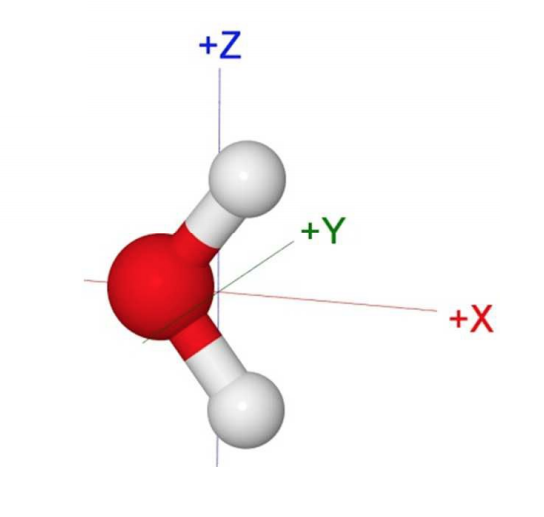
\includegraphics[width=0.6\linewidth]{Figures/System/initial_pos.png}
     \caption{Diagram illustrating the slight offset in the x-direction for the water molecule. )Adapted from [\textbf{DOI: 10.1039/C7CP06472A}].)}
     \label{fig:init_pos}
 \end{figure}
 
 In addition, reference is also made to the standard initial position. This positions implies two things. First, the dipole moment of the water molecule is parallel to the x-axis and points towards a beryllium atom. Second, due to the distribution of the charge, a slight shift in the negative x-direction is made. Figure \ref{fig:init_pos} demonstrates both of these characteristics. (Here, the (2a) Wyckoff position is taken to be the origin.) When the water molecule is rotated, it is rotated counter-clockwise about the z-axis.
 
 
\chapter{Structural Optimization}
\label{ch:struct_opt}

    \section{Introduction}
    
    The following chapter describes the various procedures used to determine an average description of the geometry of extra-framework water molecules as a function of fill. First, the volume of the supercell is optimized through a Birch-Murnaghan equation of state fitting in Section \ref{sec:eos}. Then, an assumption implemented in existing studies is tested in Section \ref{sec:da} (i.e. decoupling of the water molecule from the beryl framework) before internal relaxations of the supercell are carried out in various configurations in Section \ref{sec:geo_opt}.
    
    For each of the three sub-processes mentioned above, relevant background information, procedures, computational details, and analyses are provided. As each sub-process builds upon the previous' results, the final results and conclusions of this chapter are highlighted at the end of Section \ref{sec:geo_opt}.
    
    \section{Equation of State}
    \label{sec:eos}
        \subsection{Background Information}
        
            An equation of state describes the relationship between thermodynamic properties of a system. For instance, the Birch-Murnaghan equation of state, as described in detail in \textbf{[CITE: ((bmeos)) PRB 70,224107]},
            
            \begin{equation}
            \label{eq:bm_eos}
                E(\eta) = E_0 + \frac{9B_0V_0}{16}\left(\eta^2 -1\right)^2\left[ B'_0 \left(\eta^2-1\right) -4\eta^2\right] \text{ with } \eta = \left(\frac{V}{V_0}\right)^{1/2}
            \end{equation}
            
            \noindent relates the optimum volume $V_0$, the bulk modulus $B_0$, the first derivative of the bulk modulus $B'_0$, and the energy of the system $E$ as a function of current volume $v$. (Or, rather here, the normalized volume $\eta$ is used.)
            
            Equation \ref{eq:bm_eos} suggests a technique for determining the aforementioned thermodynamic quantities by calculating the energy of a system at various scaled volumes, which is outlined below.
        \subsection{Procedure}
        
        The following is a general procedure for fitting any equation of state, such as Eq. \ref{eq:bm_eos}. First, an initial "guess" structure $\sigma_g$ is acquired, typically from theory or experiment, with volume $V_g$. Using this structure, an ensemble of structures $\sigma_i$ with volume $V_i$ are constructed such that
        
        \begin{equation}
        \label{eq:ensem_eos}
            V_i \in \{ V_i : (1-x)V_g \le V_i \le (1+x) V_g \},
        \end{equation}
        
        \noindet for $x<1$. The initial structure $\sigma_g$ should be such that the set $\{V_i\}$ corresponds to volumes in neighborhood of $V_0$. Using each corresponding structure, the energy is calculated $E_i(V_i)$ via a self-consistent run. Finally, the resulting data is fit to Eq. \ref{eq:bm_eos} and the relevant optimized parameters are extracted.
        
        \subsection{Computational Details}
        
            For the beryl-water system, the set of $\{ V_i\}$ was sampled first in a course-grained manner with $8.7 \le a \le 9.6$ \angstrom  and $\Delta a = 0.1$ \angstrom. Then, a fine-grain scan is performed with $9.20 \le a \le 9.38$ \angstrom with $\Delta a=0.01$ \angstrom. Here, $a$ is the length of lattice vector $\Vec{a}$, which is related to the volume via
            
            \begin{equation}
                V(a) = \frac{\sqrt{3}}{2} a^2 c \text{ with } \frac{c}{a} = 0.998
            \end{equation}
            
            \noindent for beryl.
            
            The standard self-consistent calculator as outlined in \textbf{MAKE CALCULATOR SECTION} is employed for the self-consistent calculations. 
            
        \subsection{Results and Conclusions}
        
        \begin{figure}
            \centering
            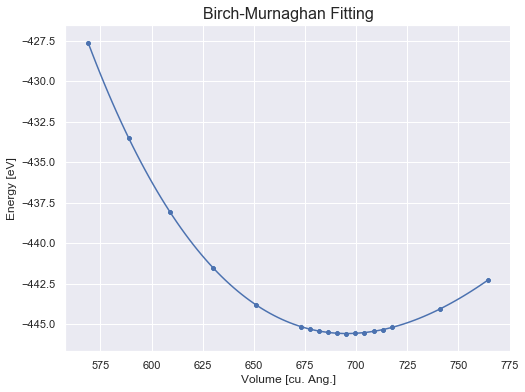
\includegraphics[width=0.8\linewidth]{Figures/System/eos.png}
            \caption{The calculated energies $E_i(V_i)$ are shown with the accompanying Birch-Murnaghan equation of state fit. The optimized volume is $V_0=695.50$ \angstrom$^3$. See text for literature comparison.}
            \label{fig:eos_fit}
        \end{figure}
        
        \begin{table}[]
            \centering
            \begin{tabular}{c|c|c}
                Observable & Value & Experiment \textbf{[CITE: eosfit]} \\
                \hline
                \hline
                $V_0$ [\angstrom$^3$] & 695.39 & $675\pm0.1$ \\
                $B_0$ [eV/\angstrom$^3$] & 1.1249 & $1.1 \pm 0.01$ \\
            \end{tabular}
            \caption{The optimized volume and bulk modulus as extracted from the fit in Fig. \ref{fig:eos_fit} are compared to literature values. See text for analysis.}
            \label{tab:eos_compare}
        \end{table}
        
        The results from the fitting are depicted in Fig. \ref{fig:eos_fit} and compared to literature values in Table \ref{tab:eos_compare}. The calculated optimized volume of $V_0 = 695.39$ \angstrom$^3$ is in good agreement with the literature value of $V=675\pm0.1$ \angstrom$^3$, especially considering that the literature values are determined at ambient temperature and pressure. 
        
        Moving forward, the cell volume will be fixed to $V=695.39$ \angstrom$^3$.
    \section{Decoupling Assumption}
    \label{sec:da}
        \subsection{Background Information}
            As previous work has demonstrated, there is no appreciable difference in geometry, potential map, or vibrational frequencies in terms of different exchange-correlation functionals, both with and without dispersion corrections \cite{vibr_states}. Effectively, this allows the crystal framework to be viewed as producing a static potential well in which the extra-framework water molecules interact. While this assumption is definitely ideal in terms of computational cost due to the relatively large number of ions and electrons in the beryl unit cell, this assumption needs to be explicitly tested before performing the geometry optimization.
            
            To this end, in the following the results of relaxing the full crystal-water system are compared to those obtained when the beryl framework is held fixed and only the water molecule is allowed to relax. Additionally, two different energy difference tolerances for self-consistency are tested.
        \subsection{Procedure}
            To begin, a single water molecule is added to the unit cell of beryl in the standard position. Such a system has a fill factor of 50\%. For each energy difference tolerances, positional degrees of freedom for both beryl and the water molecule are allowed to relax---this is referred to as the \textit{full} relaxation. Then, the beryl ions are held fixed, and only the water molecule ions are allowed to relax---this is referred to as the \textit{selective} relaxation.
            
            To compare the two relaxation schemes, the difference in position of each ion between the full and selective relaxations are calculated. By looking at both the average displacement and the maximum displacement between ions, the validity of the decoupling assumption can be determined. Additionally, the average of the water molecule bond lengths and the OHO-angle are compared for both schemes. Again, assuming the decoupling assumption holds, there should be no appreciable difference in the geometry parameters of the water molecule.
        \subsection{Computational Details}
            For both the full and selective relaxation, the relaxation calculator is used. The relaxations are performed with EDIFF set to $10^{-4}$ and $10^{-5}$. After both relaxations have been performed for each energy difference tolerance, the Atomic Simulations Environment \textbf{[CITATION]} is used to calculate the difference in ionic positions for each atom $\Delta r_i$. From the set of all ionic position differences $\{\Delta r_i \}$, the average displacement $\langle \Delta r \rangle$ and maximum displacement $\Delta r_\text{max}$ are determined. Additionally, the average of the two OH bond lengths $\langle r_\text{OH} \rangle$ and the OHO angle $\theta$ are determined for both relaxation schemes.
            
            To test the convergence of the calculations, the ratios of the water geometry parameters for each energy difference tolerance are calculated, with a ratio near unity indicating that there is no significant difference with respect to the energy difference tolerances. Finally, the ratios of the average OH bond and OHO angle for the full and selective relaxations are compared, again with a ratio near unity indicating that the decoupling assumption holds.
        \subsection{Results and Conclusions}
        
        \begin{figure}
             \centering
             \begin{subfigure}[t]{0.45\textwidth}
                 \centering
                 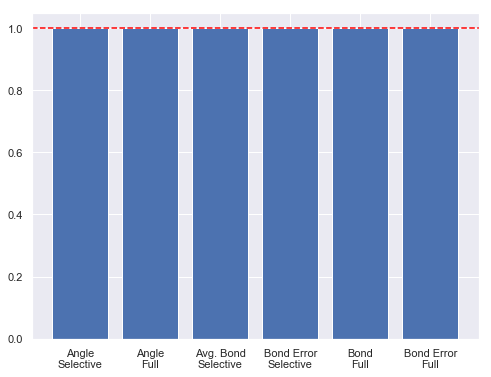
\includegraphics[width=\textwidth]{Figures/System/ediff_geom_ratios.png}
                 
                 \label{fig:ediff_geom_ratios}
             \end{subfigure}
             \hfill
             \begin{subfigure}[t]{0.45\textwidth}
                 \centering
                 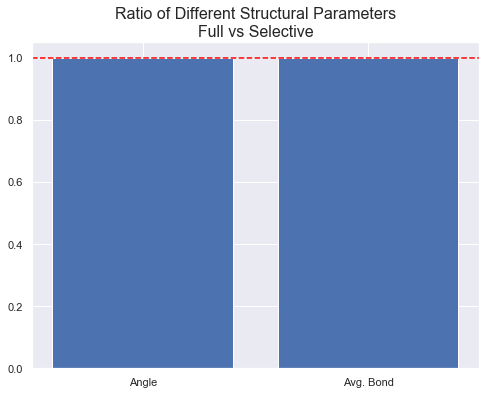
\includegraphics[width=\textwidth]{Figures/System/selective_v_full_geom_params.png}
                 \label{fig:selective_v_full}
             \end{subfigure}
                \caption{Decoupling assumption results. The red, dashed line denotes unity. (Left) The ratio of certain geometry parameters (and associated errors where appropriate) as calculated under energy difference tolerances $10^{-4}$ and $10^{-5}$. (Right) The ratio of OHO angle and average of the two OH bond lengths for the water molecule under the full and selective relaxation schemes with energy difference tolerance of $10^{-4}$. See text for full analysis.}
                \label{fig:decouple_assumption}
        \end{figure}
        
        The decoupling assumption results are summarized in Fig. \ref{fig:decouple_assumption}. Starting with the left sub-figure therein, it is clear that there is no measurable difference between the relevant geometry parameters in terms of energy stopping tolerance. Specifically, each observables ratio is nearly unity. It is therefore reasonable to conclude that the larger energy difference tolerance of $10^{-4}$ is suitable to use moving forward.
        
        \begin{table}[]
            \centering
            \begin{tabular}{c|c|c}
               Tolerance  & $\langle \Delta r \rangle$ & $\Delta r_\text{max}$  \\
               \hline
               \hline
                $10^{-4}$ & $0.008\pm 0.001$ & $0.031$  \\ 
                $10^{-5}$ & $0.010\pm0.001$& $0.033$ \\ 
            \end{tabular}
            \caption{The average difference in position over each ion and maximum difference in position between the two relaxation schemes for different energy difference tolerances. All distance measurements are in Angstroms.}
            \label{tab:ediff_r_diff}
        \end{table}
        
        Finally, to test the decoupling assumption the average OH bond length and OHO angle for both the full and selective relaxations with energy difference tolerance $10^{-4}$ are compared via their ratios in Fig. \ref{fig:decouple_assumption} (right). Again, both geometry parameters are nearly unity, suggesting there is no significant difference in the water molecule geometry between the two relaxation schemes. Furthermore, as shown in Table \ref{tab:ediff_r_diff}, both the average displacement and maximum displacement of the ions under the two relaxation schemes is significantly small compared to the length of the lattice vectors ($<1\%$ in both cases). 
        
        Therefore, the validity of the decoupling assumption is affirmed and will be implemented for the remainder of the study.
    \section{Geometry Optimization}
    \label{sec:geo_opt}
    
    With the validity of the decoupling assumption, and corresponding selective relaxation scheme, the geometry of the water molecules can be determined as a function of fill and rotation. Specifically of interest are the OH bond length and OHO angle and how they change when rotated about the high symmetry point of the beryl cage. Does these geometric parameters have a well-defined, meaningful average value? How do these parameters vary when the relative angle between extra-framework water molecules change? The remainder of this chapter sets out to answer those questions.
    
        \subsection{Procedure}
        
        \begin{figure}
            \centering
            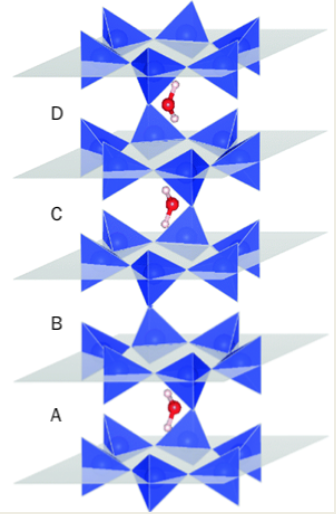
\includegraphics{Figures/System/geometry_supercell.png}
            \caption{Depiction of the supercell, with labeled cages A-D, used for the geometry optimization as outlined in the text. [\textbf{Adapted from 10.1039/c7cp06472a}]}
            \label{fig:geom_supercell}
        \end{figure}
        
        To start, a supercell is created by replicating the unit cell once in the c-direction, resulting in four cages, as shown in Fig. \ref{fig:geom_supercell}. The cages are labelled, starting from the bottom-most, as A, B, C, and D. With four cages, it is possible to probe fill factor $\phi \in \{0.25,0.50,0.75,1.00 \}$. For $\phi=0.50$, there exists a degeneracy in the fills, i.e. both configurations with A \& C filled and A \& B filled correspond to the same fill factor. To make discussion herein as unambiguous as possible, the binary conventions in Table \ref{tab:fill_conventions} are used throughout. Occasionally, the water molecule that occupies a cage may be referred to by the cage label. For example, in Fig, \ref{fig:geom_supercell}, the water molecule in cage C may be referred to as water molecule C. 
        
        \begin{table}[]
            \centering
            \begin{tabular}{c|c}
               Fill  & Occupied Cages \\
               \hline
               \hline
               1000  &  A \\
               1010  &  A, C \\
               1100  &  A, B \\
               1110  &  A, B, C \\
               1111  &  A, B, C, D\\
            \end{tabular}
            \caption{The binary convention adopted to describe the different fill possibilities.}
            \label{tab:fill_conventions}
        \end{table}
        
        While the fill factor $\phi$ provides one dimension of the parameter space to explore, it does not encompass the entirety of the space. The geometry must also be probed as a function of relative angle to the beryl framework \textit{and} the relative angle between water molecules. Naturally, only a smaller subspace of this parameter space can be sampled, and said subspace is outlined in Table \ref{tab:param_subspace}.
        
        For example, for fill 1110, molecule C is held fix, while molecule A is rotated through 12 rotations totaling $2\pi$, and for each rotation of A, molecule B is also rotates through 12 rotations totaling $2\pi$. In all, $12^2 = 144$ configurations are sampled for this fill. Also, for fill 1111, molecules A-C and B-D are pairwise ferroelectrically coupled, and therefore rotate together. 
        
        The above demonstrates the difficulty of adequately sampling this parameter space, especially considering the expense of these calculations (approximately 8 hours per configuration running on 16 cores). Given more resources, a greater sample size would be ideal, specifically increasing the number of rotations. It may also help optimization if the rotation angle were decreased to encompass only the asymmetric unit of the crystal.
        
        In addition to performing the above procedure with the water molecules in the beryl framework, the same is carried out on water molecules in the same configurations in the absence of the beryl crystal. In other words, the spacing and rotation of the water molecules is the same, but the calculations are carried out in vacuum. This allows for investigation of how the beryl framework affects the geometry, if at all.
        
        \begin{table}[]
            \centering
            \begin{tabular}{c|c|c|c}
                Fill & No. Rotations & Rotation Angle  & Rotated Molecules  \\
                \hline
                \hline
                1000 & 30 & $2\pi$ & A \\
                1010 & 12 & $2\pi$ & A, C \\
                1100 & 12 & $2\pi$ & A, B \\
                1110 & 12 & $2\pi$ & A, B \\
                1111 & 12 & $2\pi$ & A-C,B-D \\
            \end{tabular}
            \caption{Outline of the parameter subspace sampled as part of the geometry optimization. See text for details.}
            \label{tab:param_subspace}
        \end{table}
        
        \subsection{Computational Details}
        
        For each configuration in Table \ref{tab:param_subspace}, the selective relaxation scheme as outlined in \ref{sec:da} is used. After the relaxation, the relevant geometric measurements are made using ASE. 
        
        \subsection{Results and Conclusions}
        \label{sec:geom_opt}
        
        \begin{figure}
            \centering
            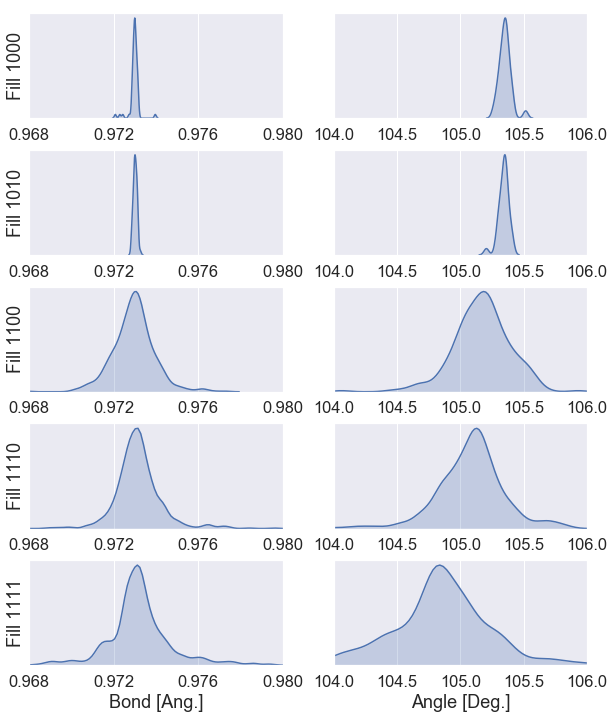
\includegraphics[width=0.85\linewidth]{Figures/System/geom_kdes.png}
            \caption{Kernel density estimates for the OH bond lengths (left) and OHO angles (angles) by fill. }
            \label{fig:geom_kdes}
        \end{figure}
        
        Figure \ref{fig:geom_kdes} shows the kernel density estimates for the OH bond lengths and OHO angles. Each subplot represents the population density of the sampled set. Immediately clear is the fact that there is an effect of fill on the geometry of the water molecules, as evident by the qualitative difference in shape of the population densities. In any case, for each, there is a well-defined peak, suggesting that an average geometry per fill is meaningful. However, the variance of the population density is directly proportional to the fill, suggesting that rotation does have some effect on the geometry. 
        
        
        
        \begin{figure}
            \centering
            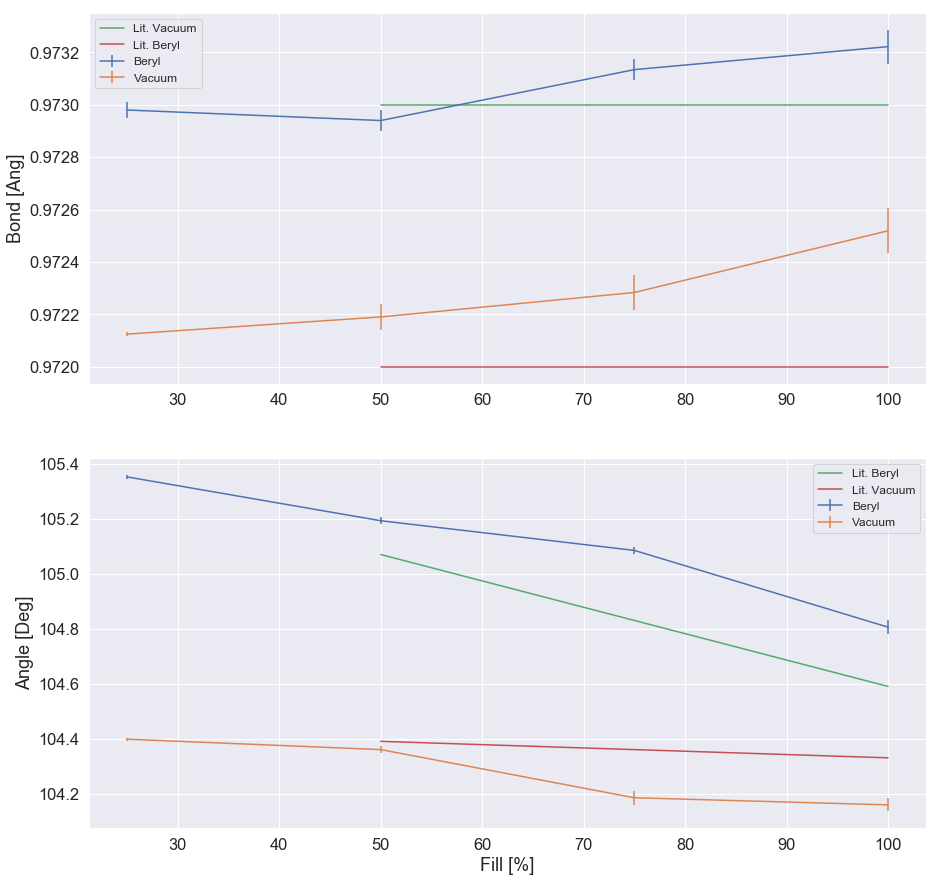
\includegraphics[width=0.85\linewidth]{Figures/System/geom_results.png}
            \caption{The average OH bond length (top) and OHO angle (bottom) per fill factor are compared to literature values, when possible. Error bars represent the standard errors of the mean.}
            \label{fig:geom_results}
        \end{figure}
        
        For a more quantitative analysis, the averages and standard errors of the mean are used as shown in Fig. \ref{fig:geom_results}. Here, the populations (and therefore, results) for fills 1010 and 1100 are combined. 
        
        From both the OH bond length and OHO bond angle (blue line), it is clear that there is an effect from the fill factor on the geometry of the water molecule. Specifically, as more water molecules are added, the OH bond lengthens slightly, while the OHO angle decreases. Additionally, an effect from the beryl crystal is evident (orange vs. blue line) in that the beryl has a \textit{dilating} influence on the water molecule---the OH bond length systematically increases and the OHO angle systematically expands. 
        
        As a benchmark, these results are acceptably compared to the work done in \cite{vibr_states} (green and red lines). Here, the systematic differences can be explained by the procedure followed in said work. Instead of relaxing the water molecule under the optimized beryl geometry, the beryl geometry was set to match an experimental sample to which they were comparing their computational results. Additionally, only fill factors $\phi = 0.50, 1.00$ were investigated. 
        
        Moving forward, the fill specific geometries, as shown in Fig. \ref{fig:geom_results}, are used. 
        
        \paragraph{Outlook}
        To improve upon these parameters, a larger subspace of the parameter space should be investigated. Additionally, changing the size and shape of the unit cell---and thus the fill configurations that correspond to certain fill factors $\phi$---and investigating the average geometry would be of interest as well. Notebly, what happens if the supercell is created by replicating the unit cell along the a- or b-directions? 
\chapter{Potential Map}

With an average geometry in-hand, the potential map for the water molecules rotating about the high-symmetry point can be investigated, which is the primary focus of this chapter. To begin, a broad sweep is conducted to confirm energy convergence, verify that the antiferroelectric coupling is energetically favorable, and to determine a smaller range for a fine sweep that captures all of the interesting features. 

With an acceptable smaller range for the fine sweep identified, a fine sweep is carried out with antiferroelectric coupling both within the beryl framework and in vacuum. Furthermore, a fine sweep potential map is measured in vacuum with the beryl-based water molecule geometry as found in the previous chapter. 

In the final subsection, the differences in the fine sweep potential map are analyzed to determine (a) if the \textit{interesting} features of the potential maps are products of interaction in the water-beryl or water-water subsystems and (b) what the contribution is of the water-beryl subsystem interactions to the total potential map.

    \section{Motivation for Investigation}
    Before beginning, however, it is important to highlight exactly why the high-symmetry potential map is worth investigating.
    \textbf{WRITE THIS SECTION}. Different assumptions in literature, good point of comparison, etc.

    \section{Broad Sweep}
    Like one would do when surveying a new region, a broad sweep is first carried out to set bearings, test a assumptions, and begin to understand how both fill and rotation of the water molecules affects the energetics of the system. 
        \subsection{Energy Convergence Test}
        \label{sec:en_conv_test}
        \paragraph{Procedure} As was done with the structural optimization, the convergence of the relevant parameter--here, potential energy--is first tested. In previous works, energy barriers for the water molecule librations are reported to be fraction of meV \cite{vibr_states}. To recall, an energy difference tolerance of $10^{-4}$ eV for the structural optimization. Again, for reasons of computational cost, using this tolerance is ideal, but it is on the order of the features intended to be measured. Therefore, the potential map under this energy difference tolerance is compared to that obtained under a tolerance of $10^{-6}$ eV. 
        
        For the larger tolerance, the configuration for fill 1010 is used. The two extra-framework water molecules are coupled ferroelectrically---meaning the relative angle between molecules vanishes at all times---and starting from the standard position, are rotated through $\pi$ radians in steps of $\Delta \theta = \pi/150$. The resulting potential map is then inspected (see Fig. \ref{fig:pmap_convergence}) to determine a slightly smaller rotation range for the smaller tolerance that still maps the features of interest, since the computation time for said smaller tolerance is significantly longer. Using this smaller range of $\pi/3$ radians with the same $\Delta \theta$, the ferroelectrically coupled water molecules are again rotated, and the potential map is measured.
        
        The comparison of these maps is carried out via the ratio of the energies for each angle $\theta \in \{0,\pi/3\}$. Again, assuming that the results are not significantly difference, the ratio should approach unity for each rotated configuration.
        
        \paragraph{Calculation Details} For each rotated configuration, the standard self-consistent calculator is used, with the only difference being the energy difference tolerance EDIFF as out discussed above.
        
        \paragraph{Results and Analysis}
        
        \begin{figure}
            \centering
            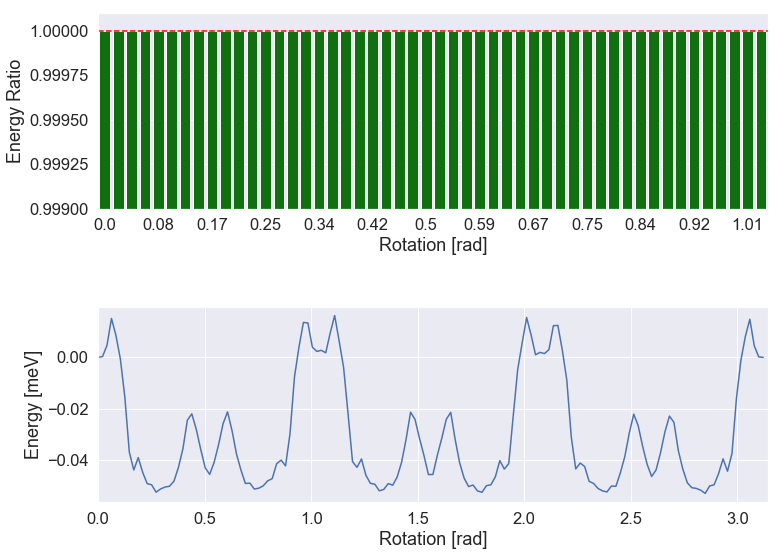
\includegraphics[width=0.8\linewidth]{Figures/System/pmap_convergence.png}
            \caption{The results for the energy convergence test. (Top) The ratio of the energies calculated under both energy difference tolerance for each rotated configuration. The dashed, red line indicated unity. (Bottom) The broad sweep potential map under energy difference tolerance $10^{-4}$ eV. See text for analysis. }
            \label{fig:pmap_convergence}
        \end{figure}
        
        The results for the energy convergence test are shown in Fig. \ref{fig:pmap_convergence}. As evident from the top subfigure therein, no appreciable accuracy in the potential energy calculation is gained from the smaller energy difference tolerance. For each angle of rotation, the ratio is exactly unity, at least within the resolution of the graph. The larger tolerance is therefore deemed acceptably converged for purposes of calculating potential maps.
        
        The bottom subfigure in Fig. \ref{fig:pmap_convergence} shows the broad sweep potential map. Immediately, some relevant features are identifiable. Specifically, there are two sets of 6-fold degenerate local minima. The first of these two local minima appear at $\theta = n\pi/3$ for $n\in \left[0,5\right] \cap \mathbb{Z}$. These angles correspond to positions where the water molecule dipole moment is coincident with the dipole moment of a nearest neighbor water molecule. (See Fig. \ref{fig:supercell} for visual aid.) Offset from these minima by $\Delta \theta = \pi/6$ radians are the second set of local minima, which correspond to dipole coincidence amongst next-nearest neighbors. 
        
        Additionally, there exists a 12-fold degenerate global minimum in-between the two above described local minima and other shoulder features within the potential map. These will be examined in further detail under the fine sweep, along with an attempt to determine the originating interactions for said features.
        
        \begin{figure}
            \centering
            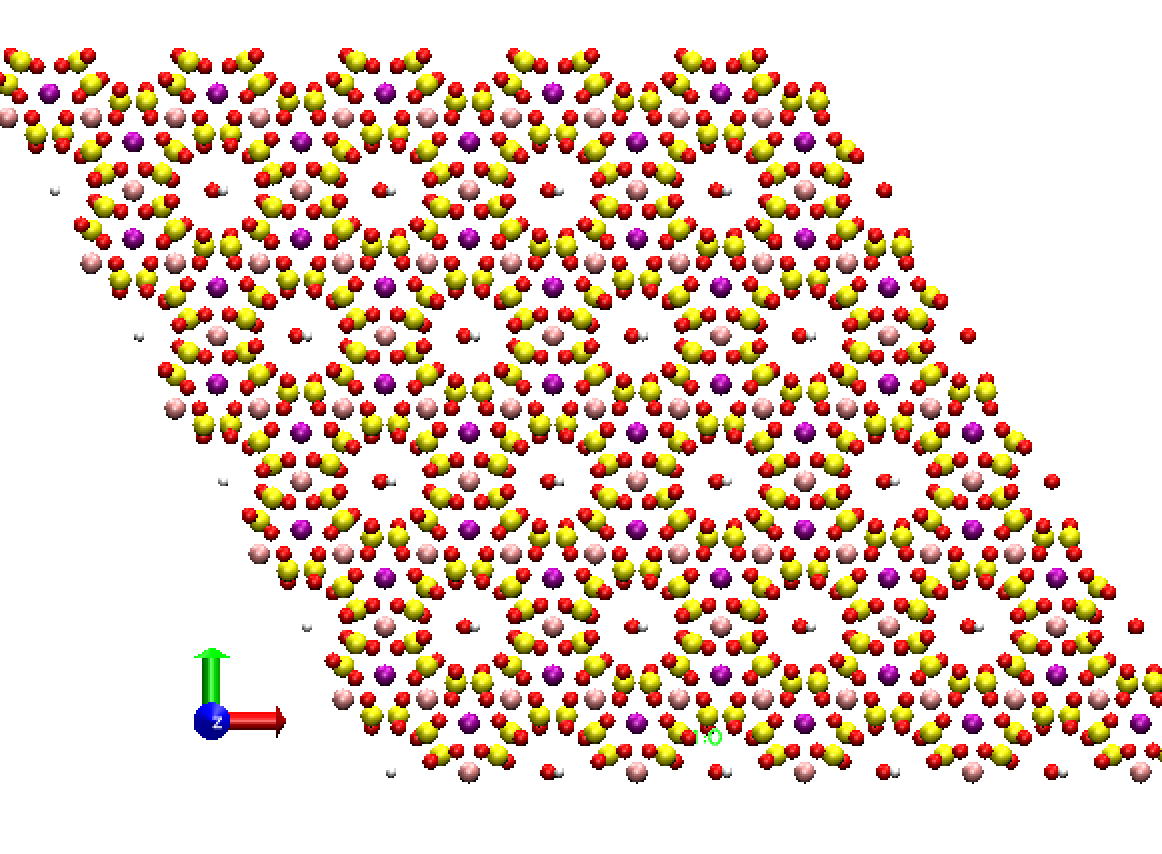
\includegraphics[width=0.8\linewidth]{Figures/System/supercell.png}
            \caption{Large supercell of ferroelectrically coupled fill 1010 system.}
            \label{fig:supercell}
        \end{figure}
        
        \paragraph{Conclusions} The above results are consistent with existing studies that utilized the potential map in some fashion \cite{vibr_states} [\textbf{CITE OTHER PMAP ARTICLE}] in the sense that there does exist a 6-fold degenerate local minimum that corresponds to symmetric rotation configuration about the high-symmetry point. However, thus far an ambiguity has been raised, because it is not clear \textit{which} of the two 6-fold degenerate minima the previous works are referring. Once a fine sweep is conducted, energy barriers can be measured, and hopefully this ambiguity can be lifted.
        
        For the remainder of the broad sweep investigation and in the interest of speeding up data set collection times, a smaller rotation of $\pi/3$ radians is deemed appropriate to capture the three minima and other relevant features. 
        
        \subsection{Relative Angle Test}
        \label{sec:rel_ang_Test}
        
        \paragraph{Background Information }Moving forward, choices need to be made to limit the portion of the parameter space that is sampled due to resource limitations. Since the ultimate goal is to develop a parameterized force field that can capture the groundstate interactions of the extra-framework water molecules, limiting the calculated potential maps to those that correspond to the most energetically favored state is one such choice. If the contributions from the framework crystal are truly of the static variety, then thinking of the water-water subsystem as two identical, interacting classical dipoles in vacuum is a useful heuristic. If said dipoles are interacting in the same fashion as the two water molecules in the crystal, the only relevant degree of freedom is rotation about the c-axis, and the interaction is described by
        
        \begin{equation}
        \label{eq:dip_interaction}
            V(\theta) = k\frac{p^2\cos \theta}{r_0^3},
        \end{equation}
        
        \noindent for some constant of proportionality $k$, dipole moment $p$, separation distance $r_0$, and relative angle $\theta$. Equation \ref{eq:dip_interaction} is minimized when $\theta = \pi$, or when the two dipoles are antiferroelectrically coupled. 
        
        \paragraph{Procedure} Sticking with the fill 1010 configuration, potential maps through rotation angle $\pi/3$ radians with $\Delta \theta = \pi/90$ are calculated where the relative angle between the water molecules $\alpha$ is varied. The relative angles investigated are $0 \le \alpha \le \pi$ in increments of $\Delta \alpha = \pi/6$.
        
        \paragraph{Calculation Details} As before, the standard self-consistent calculator is used for each configuration listed above.
        
        \paragraph{Results and Analysis}
        
        The results of the relative angle test are given in Fig. \ref{fig:pmap_rel_angle}. Immediately, it's clear that the potential maps are qualitatively equivalent not only to each other, but also to the results of the convergence test (Fig. \ref{fig:pmap_convergence}). Specifically, the degeneracy previously identified are present for each relative angle configuration. 
        
        \begin{figure}
            \centering
            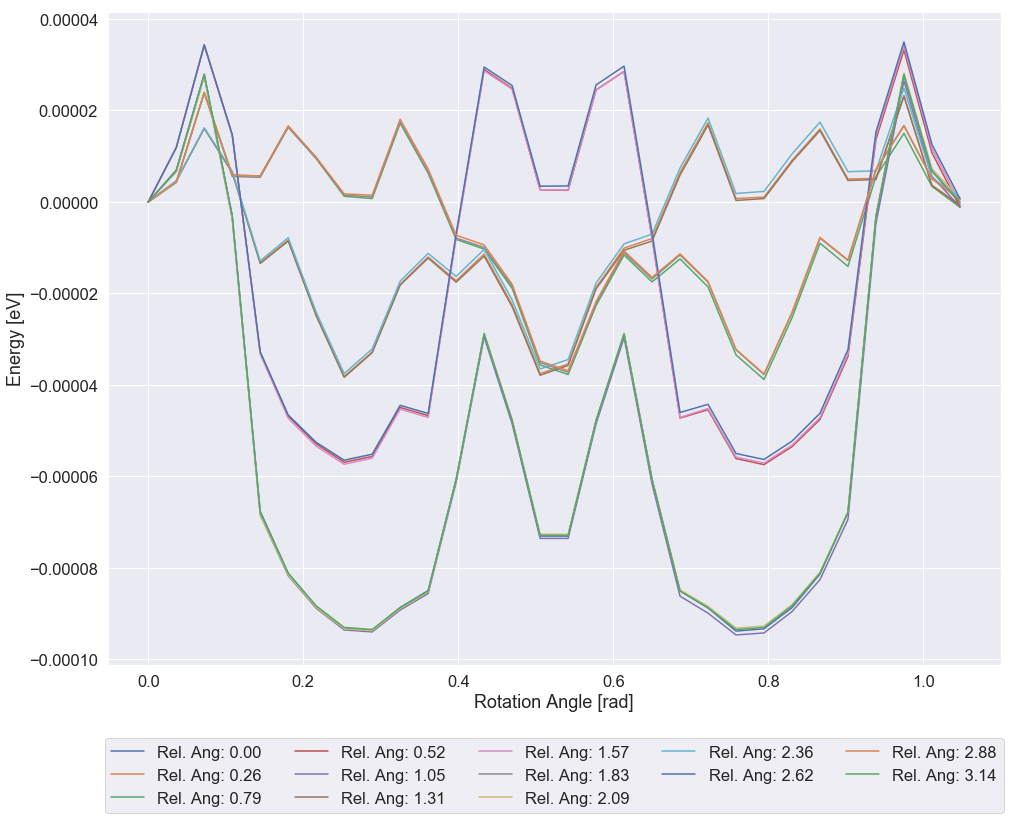
\includegraphics[width=0.9\linewidth]{Figures/System/pmap_rel_angle.png}
            \caption{The potential maps for various relative angle between water dipoles $\alpha$. See text for analysis.}
            \label{fig:pmap_rel_angle}
        \end{figure}
        
        Turning now to the differences between the relative angle potential maps, it is clear from inspection that the antiferroelectrically coupled configuration is the most energetically favorable. Furthermore, the potential map appears to experience a non-linear, negative shift as relative angle increases. There also appear to be differences in the \textit{topology} of the potential maps. 
        
        A more quantitative analysis of the changes described above entails comparing the results to (\ref{eq:dip_interaction}) by answering the question, how does the potential map behave as molecule A is held fixed while molecule C rotates? To answer this question, vertical line cuts of Fig. \ref{fig:pmap_rel_angle} are made using the following procedure for each rotation angle $\theta_i$. The energy difference between $E(\theta_i,\alpha_j)$ for relative angle $\alpha_j$ and $E(\theta_i,0)$ is determined for each $\theta_i$ and $\alpha_j$. Then, the average is taken over all $\theta_i$, resulting in an average description of the energy as a function of relative dipole angle $\alpha$ that should be approximated by (\ref{eq:dip_interaction}). The results are shown in Fig. \ref{fig:relative_angle_fit}. Here, the function is fit by hand to 
        
        \begin{equation}
            E(\alpha) = A \sin(\omega \alpha),
        \end{equation}
        
        \noindet with amplitude $A = -0.88$ meV and frequency $\omega = \pi/6$. The function was fit by hand due to the difficulties of fitting a sinusoidal function only one-half wavelength's worth of data. Even with such a rudimentary fit protocol, though, it is clear that the data agrees reasonable well with (\ref{eq:dip_interaction}), with deviations (specifically below 1.0 radians) being attributed to dipole-framework and higher order dipole-dipole interactions that are not captures by the heuristic assumption. The need for error bars---representing the standard error of the mean---further suggests that the dipole-framework and higher order dipole-dipole interactions influence the potential map topology. Put differently, the distinguishable features of the potential map should vary with relative angle.
        
        \begin{figure}
            \centering
            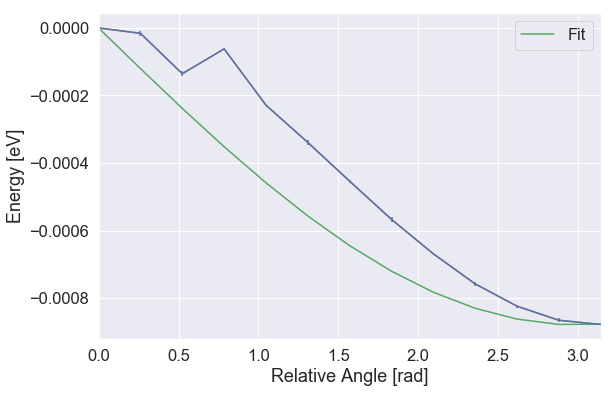
\includegraphics[width=0.9\linewidth]{Figures/System/relative_angle_fit.png}
            \caption{The average energy as a function of relative angle $\alpha$ is compared to a sine function. See text for details.}
            \label{fig:relative_angle_fit}
        \end{figure}
        
        This variation is captured when each potential map in Fig. \ref{fig:pmap_rel_angle} is zeroed relative to the energy in the initial configuration, as shown in Fig. \ref{fig:zeroed_relative_angle_pmap}. In general, the two 6-fold degeneracies and one 12-fold degeneracy are visible for each relative angle, but the energetic of these features varies with relative angle. 
        
        \begin{figure}
            \centering
            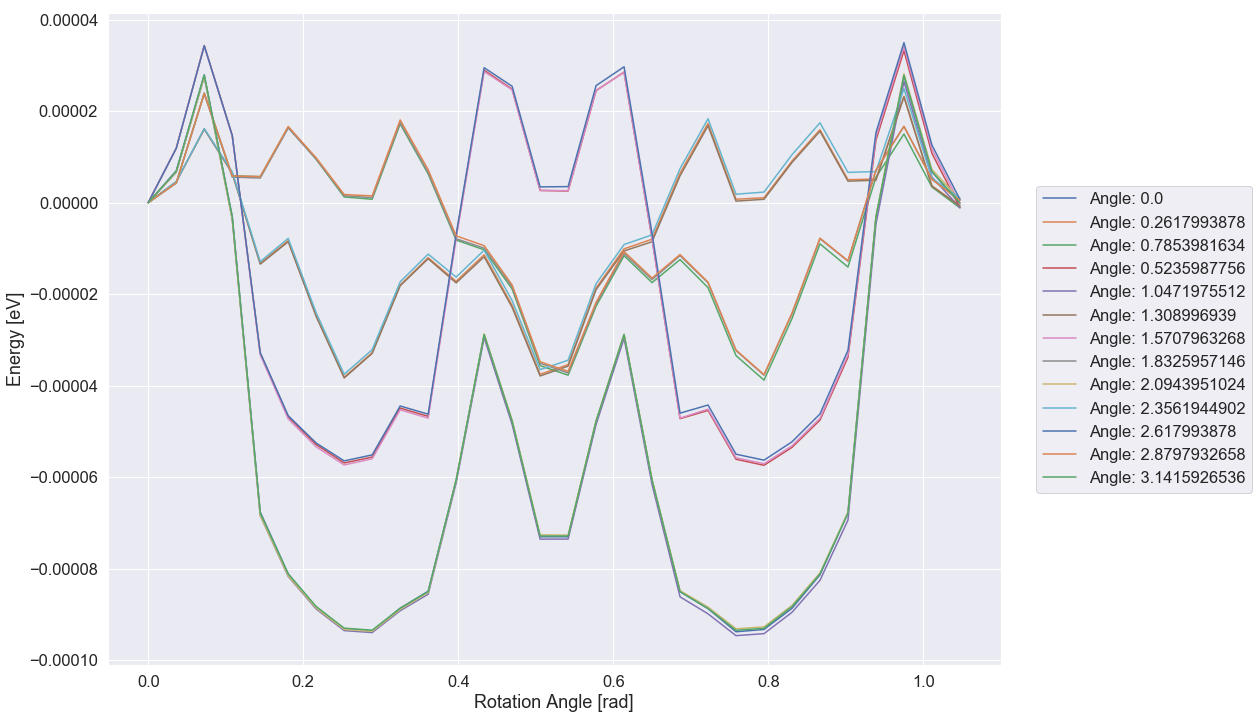
\includegraphics[width=0.9\linewidth]{Figures/System/pmap_zeroed_relative_angle.png}
            \caption{Relative angle potential maps zeroed relative to the energy of the initial configuration.}
            \label{fig:zeroed_relative_angle_pmap}
        \end{figure}
        
        \paragraph{Conclusions} Finally, the antiferroelectrically coupled configuration, as predicted by the heuristic assumption, is in fact the most energetically favorable and allows for a reduction in parameter space. Using this reduced parameter space, the effect that additional water molecules have on the potential map can be investigated by determining the antiferroelectrically coupled map for each fill configuration.
        
        \subsection{Map vs. Fill}
        \label{sec:map_v_fill}
        
        \paragraph{Procedure} Similar to the relative angle test procedure, potential maps are calculated for each fill using antiferroelectrically coupled water molecules. The molecules are rotated through $pi/3$ radians with $\Delta \theta = pi/90$. To make a meaningful comparison between fills, each potential map is zereoed to the energy of the initial configuration.
        
        \paragraph{Calculation Details} The standard self-consistent calculated is used.
        
        \paragraph{Results and Analysis}
        
        \begin{figure}
            \centering
            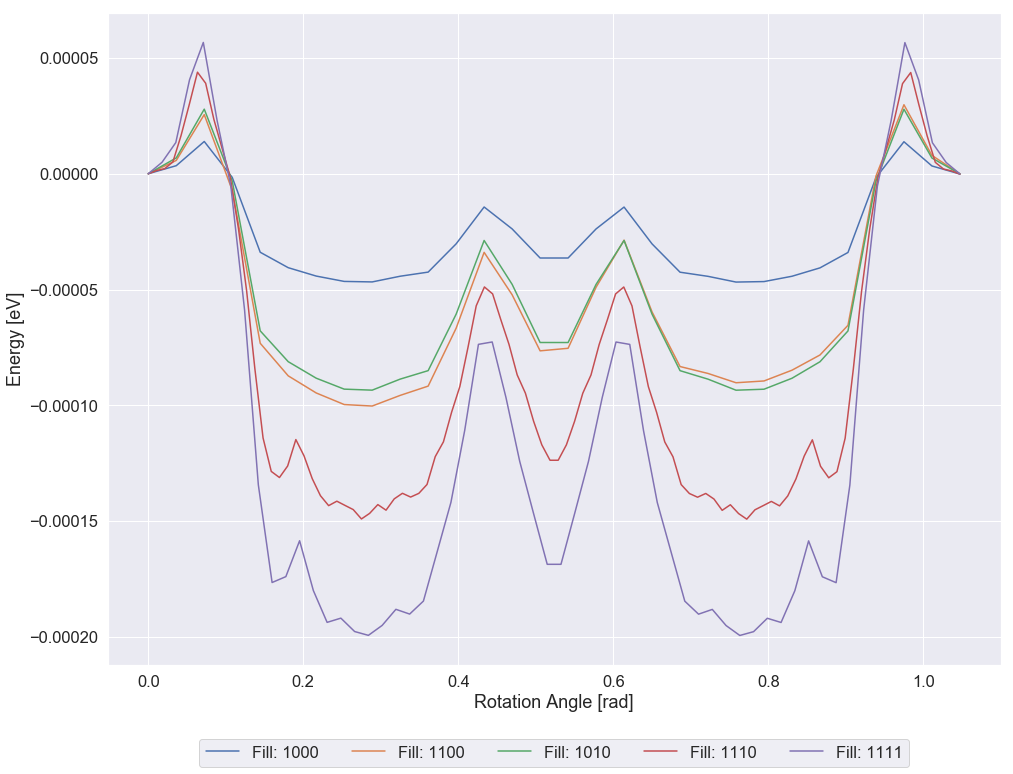
\includegraphics[width=0.9\linewidth]{Figures/System/pmap_af_broad.png}
            \caption{The antiferroelectrically coupled potential maps as a function of fill.}
            \label{fig:pmap_af_broad}
        \end{figure}
        
        Figure \ref{fig:pmap_af_broad} shows the potential maps as a function of fill. The interesting features, namely the already-described degeneracies, are evident in each fill (although some of the smaller shoulders are not visible within the resolution of the graph). As more water molecules are added, the potential wells deepen. Also, by comparing the local minima to the crystal symmetry, the minima correspond to instances when the water molecules are colinear with nearest- or next-nearest-neighbor water molecules. It is unclear at this point, however, if the features should be attributed to dipole-dipole interaction or dipole-framework interactions. The next section will attempt to probe this ambiguity by performing a fine sweep over $0\le \theta \le 0.6$ radians, which will capture all relevant features shown in Fig. \ref{fig:pmap_af_broad}. To try to disentangle the dipole-framework and dipole-dipole interactions, potential maps will also be calculated for arrays of water molecules in vacuum with the same spacing as if the crystal were present.
        
        Before moving on, however, it is also useful to look at how the average energy of the system changes as a function of fill. By averaging the total energies over configurations for each fill, the effect that adding water molecules to the crystal can be ascertained. These results are depicted in Fig. \ref{fig:pmap_avg_energy}. Here, the results for the degenerate $\phi = 0.5$ case are combined.
        
        It is clear that there is a well-defined inverse, linear relationship between the number of water molecules and the total energy of the system. It is worth remembering at this point, though, that the geometry of the crystal framework was held constant for all calculations, so the true relationship might deviated slightly from near-perfect linearity. 
        
        From fitting the data to 
        
        \begin{equation}
            y = -57.28x+14.32 \text{ with } x = \frac{n_\text{w}}{4},
        \end{equation}
        
        \noindent with number of water molecules $n_\text{w}$, the addition of each water molecule decreases the total energy by 14.3125 eV. Thus, it is energetically favorable for a beryl crystal to have every cage filled with a water molecule.
        
        It would be interesting to see how Fig. \ref{fig:pmap_avg_energy} would look using a larger unit cell with greater fill degeneracies, since such a curve would more accurately describe nature. Such large unit cells would be extremely expensive to calculate and would require greater computational resources than were available at time of research.
        
        \begin{figure}
            \centering
            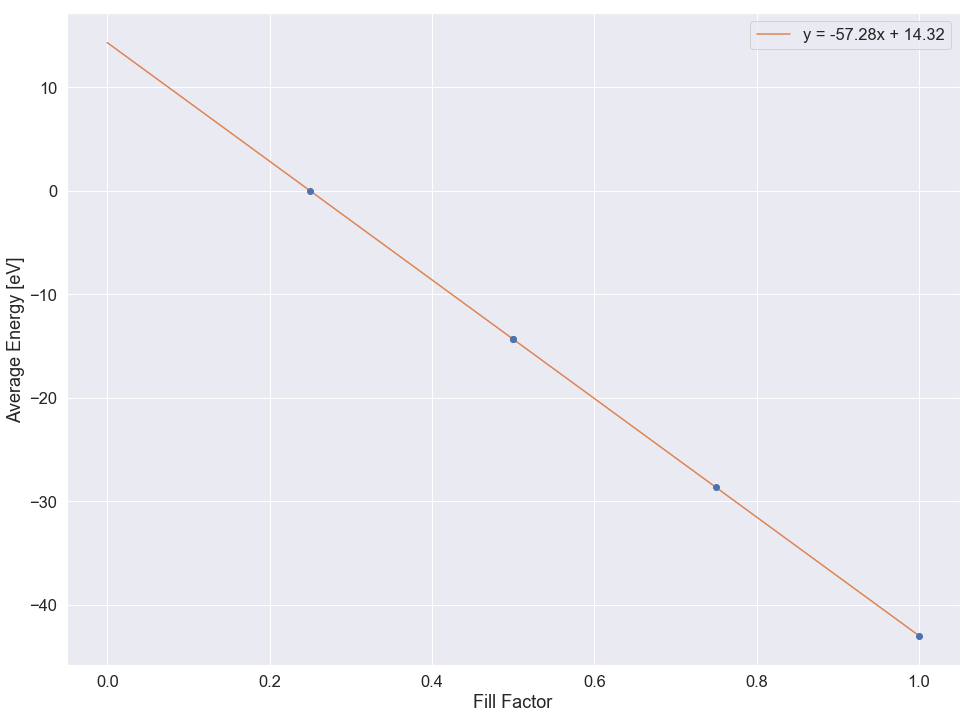
\includegraphics[width=0.9\linewidth]{Figures/System/pmap_broad_avg_energy.png}
            \caption{The average energy as determined by the self-consistent calculation for each fill. The error bars, which are not visible within the resolution of the graph, represent the standard-error of the mean.}
            \label{fig:pmap_avg_energy}
        \end{figure}
        
        
        
    \section{Fine Sweep}
    \label{sec:fine_sweep}
    
    The broad-sweep potential maps offer enlightening insights into the energetics of the beryl-water system but much of the results are qualitative in nature. For instance, how does the energy difference between the local minima change \textit{quantitatively} as a function of fill? Furthermore, are the distinguishable features of the potential map due to dipole-dipole or dipole-framework interactions? 
    
    \paragraph{Procedure} To answer these questions, potential maps will be calculated over a smaller range with greater resolution for two cases: (a) the water molecule arrays are within the beryl crystal and (b) the water molecule arrays are in vacuum but with the same spacing as in case (a). For case (b), potential maps will be calculated with two different water molecule geometries: (1) the vacuum geometry and (2) the beryl geometries as described in Section \ref{sec:geom_opt}. For each case, the water molecules will be antiferroelectrically coupled and rotated through $0\le \theta \le 0.6$ with $\Delta \theta = 0.01$. 
    
    Finally, by taking the difference between pairs of these three potential maps, an attempt is made to disentangle the dipole-dipole and dipole-framework interactions.
    
    \paragraph{Calculation Details} The self-consistent calculator is used for all calculations.
    
        \subsection{In Beryl}
        \label{sec:fine_sweep_beryl}
        
        Figure \ref{fig:pmap_fine_sweep} shows the fine-sweep potential maps as well as five critical points A-E as indicated by vertical lines. Points A, C, E are local minima while points B, D are local maxima. The critical points were determined by finding the local minimum/maximum amongst the sampled points in the neighborhood of the visually identifiable critical points. Thus, these points are approximations of the true critical points, with the accuracy improving with smaller sample frequencies. 
        
        
         \begin{figure}
             \centering
             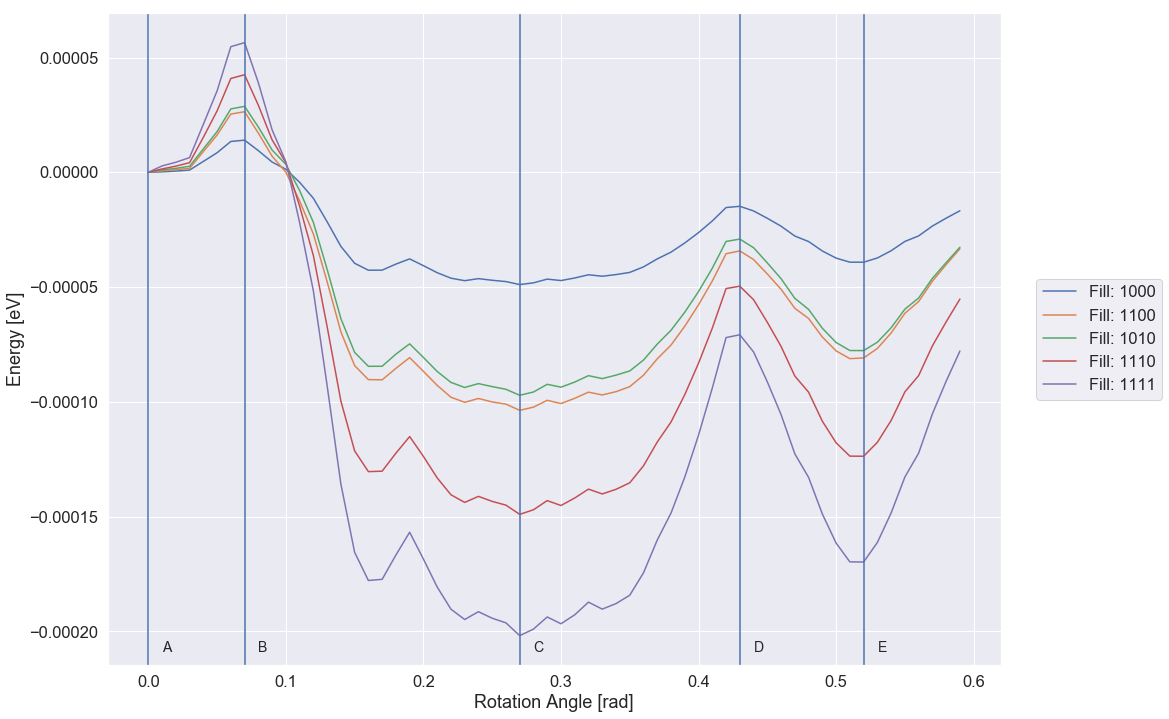
\includegraphics[width=0.9\linewidth]{Figures/System/pmap_fine_sweep.png}
             \caption{Fine-sweep potential maps for each fill with five critical points A-E identified by vertical lines.}
             \label{fig:pmap_fine_sweep}
         \end{figure}
         
         Nevertheless, quantitative information can be obtained about the effect of adding additional water molecules by comparing the energy differences between critical points, as shown in Fig. \ref{fig:pmap_cp_diff}. Here, the relative differences amongst the local minima A, C, E (respectively at points A, C, E) are compared as a function of fill, and the dilating effect of adding additional water molecules is clearly visible by the greater absolute difference in energy between all minima. 
         
         Figure \ref{fig:pmap_cp_diff} also identifies a source of systematic error in that the intercepts do not all vanish. This is possibly due to calculation-approximation systematic errors---such as tolerances, basis sets, functionals, etc.---or more likely due to the finite,small unit cell. Looking at the only degenerate case $\phi=50$, there is slight difference in the results due to the different configurations, and thus an aggregate value must be used. In the limits of an infinite unit cell and of sampling all degenerate configurations, this error would likely be eliminated. There is the possibility that the intercept may not truly vanish, though, which would indicate that some contribution from the dipole-framework exists as well.
         
         \begin{figure}
             \centering
             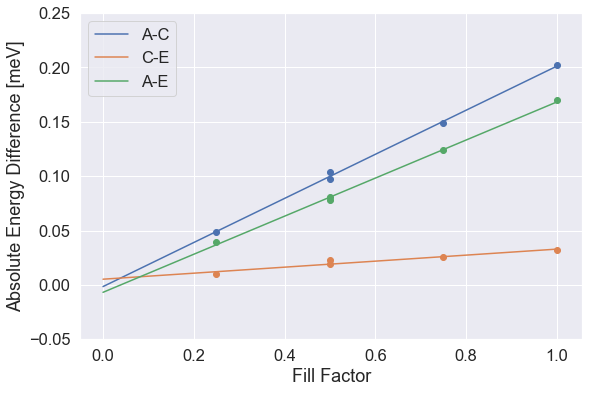
\includegraphics[width=0.9\linewidth]{Figures/System/pmap_cp_diff.png}
             \caption{The difference in energy between the local minima as a function of fill.}
             \label{fig:pmap_cp_diff}
         \end{figure}
         
         The critical point analysis may also hint at a way to dramatically improve experimental investigations of these systems. As it stands, if one wanted to conduct fill-based analysis on an observable, say dielectric response, they must first perform all necessary spectroscopic experiments before determining the fill via mass spectrometer. All the while hoping that the sample they are working with has the fill that they want. On the other hand, if some type of scattering experiment were able to resolve any of the energy differences between local minima, future researchers would be able to approximate their system's fill by performing such a scattering experiment, virtually eliminating the aforementioned experimental bottleneck.
         
         Finally, the fact that the absolute energy differences nearly all vanish suggests that the potential map features are primarily due to interactions within the dipole-dipole system. To elucidate this observation, similar analysis is performed on the vacuum potential maps.

        \subsection{In Vacuum}
        \label{sec:fine_sweep_Vacuum}
        
        Using the vacuum potential maps in Fig. \ref{fig:pmap_vacuum_comparison}, the dipole-dipole and dipole-framework interactions can begin to be disentangled. In said figure, the solid, colored line represent the potential map of an array of water molecules with spacing as if they were within the framework crystal but with the vacuum internal geometry. Because it was shown that the crystal has an effect on the geometry of the water molecule, vacuum potential maps where also calculated using the beryl internal geometry. These latter results are represented by the dotted, black lines. From inspection, it is clear that the beryl geometry slightly raises the energy systematically. but the distinguishable features remain qualitatively unchanged.
        
        \begin{figure}
            \centering
            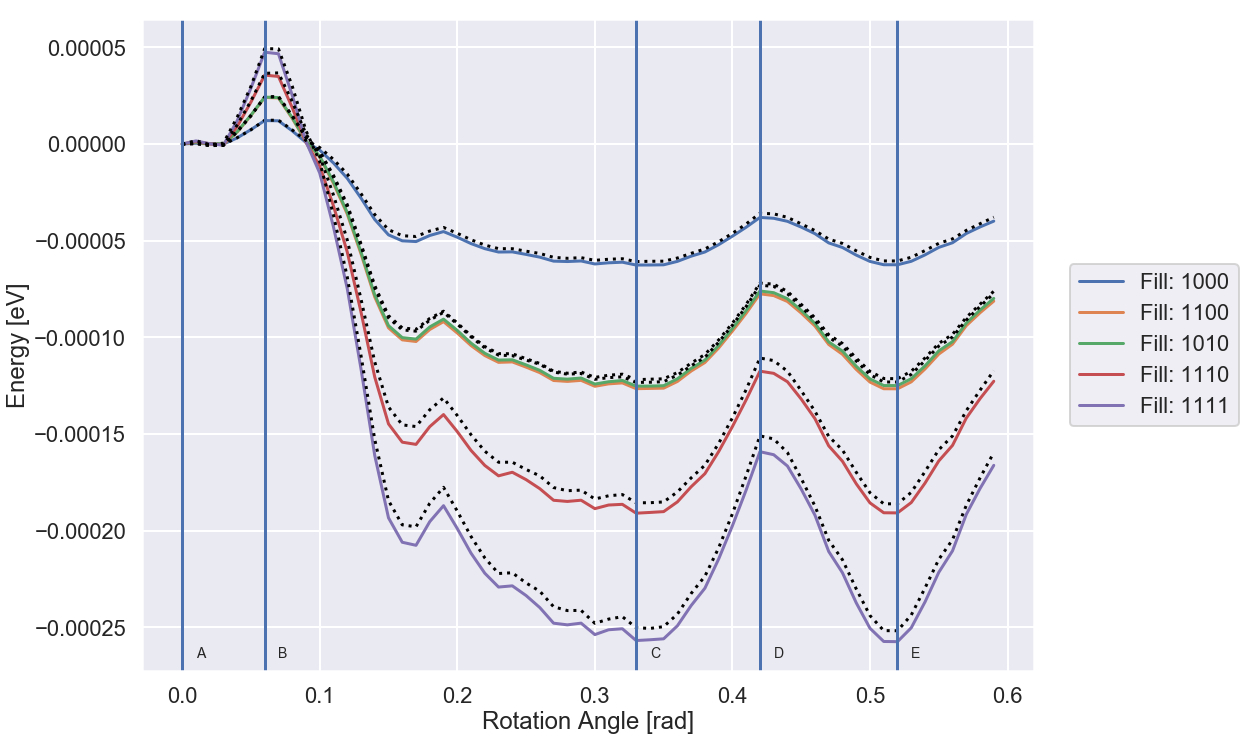
\includegraphics[width=0.9\linewidth]{Figures/System/pmap_vacuum_comparison.png}
            \caption{Potential map by fill for arrays of water molecules in vacuum. The solid, colored lines represent results for water molecules with vacuum geometry, while the black, dotted lines represent results for water molecules with beryl geometry. Critical points are identified as before.}
            \label{fig:pmap_vacuum_comparison}
        \end{figure}
        
        The critical points are determined using the same protocol as in the beryl case. It is worth noting that the angle at which these critical points occur differs from that of the beryl case. For instance, in the absence of the beryl crystal, critical point B is shifted to the left, while critical point C is shifted to the right. Since these represent a local maximum and a local minimum respectively, this suggests that the dipole-framework interactions yield a slight increase in energy. This observation will be discussed in more depth in the Difference Analysis section.
        
        \begin{figure}
            \centering
            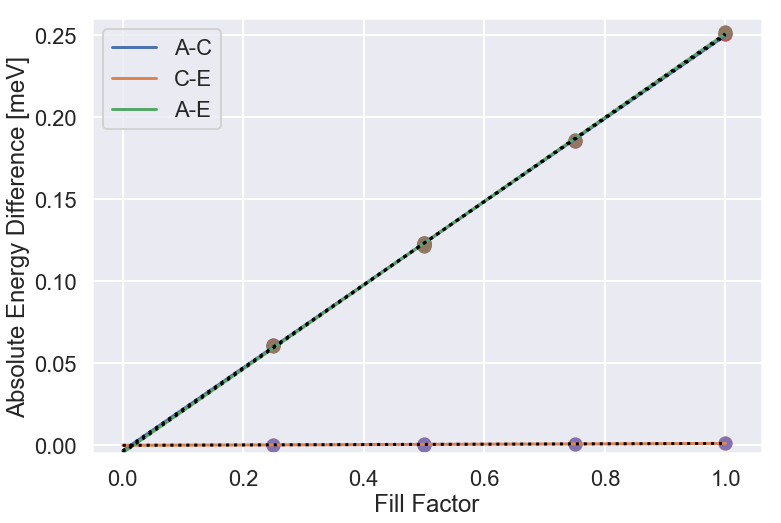
\includegraphics[width=0.9\linewidth]{Figures/System/pmap_vacuum_cps.png}
            \caption{The absolute energy differences are various critical points for the vacuum potential maps. Again, the solid, color lines represent results for vacuum-geometry water molecules, while the dotted, black lines represent the results for beryl-geometry water molecules.}
            \label{fig:pmap_vaccum_cps}
        \end{figure}
        
        Before moving on to the difference analysis, the difference in absolute energy between critical points A, C, and E is examined as in the beryl case (Fig. \ref{fig:pmap_vaccum_cps}. As mentioned in the caption, the same line-style convention is used as in Fig. \ref{fig:pmap_vacuum_comparison}. There exists no distinguishable difference between the vacuum-geometry and beryl-geometry water molecules. There is, however, a striking difference between these results and those shown in Fig. \ref{fig:pmap_cp_diff}. Namely, there is a degeneracy in the vacuum case that appears to be lifted within the present of the crystal framework. In Fig. \ref{fig:pmap_vaccum_cps}, The difference in energy between point A and points C, E are the same, while the difference between points C, E appears to vanish. This suggests that a degeneracy exists for the global minimum at points C and E. The lifting of this degeneracy supports the previous finding that the crystal acts as a non-interacting, background potential.
        
        One further point on the degeneracy here: It is known that in the case of a one-dimensional chain of spins in vacuum no phase transition occurs with respect to their alignment \textbf{[citation needed?]}. It may be this degenerate groundstate that plays a role in suppressing such a phase transition, at least in the case of water molecules with the current spacing. Since this degeneracy is lifted in the crystal framework, perhaps a one-dimension chain could exhibit a phase transition. At the very least, it warrants greater investigation.
        
        \subsection{Difference Analysis}
        \label{sec:diff_anal}
        
        There are two ways that information about that the dipole-framework interactions can be disentangled using the potential map data. The first to look at how the critical points shift in the potential map when going from the vacuum case to the beryl case, as shown in Fig. \ref{fig:cp_diff}. Both local minima A and E---corresponding to dipoles being co-linear with the nearest- and next-nearest neighbors, respectively---appear to be unchanged by the addition of the crystal framework. However, the local minimum C experiencing a significant shift to the left when the framework is included. Similarly, the local maxima B and D are both shifted to the right. Both of these shifts are consistent with a static background potential that is directly proportional to the rotation angle over the range calculated. Considering the six-fold symmetry of the system, this background potential likely also exhibits a six-fold potential.
        
        \begin{figure}
            \centering
            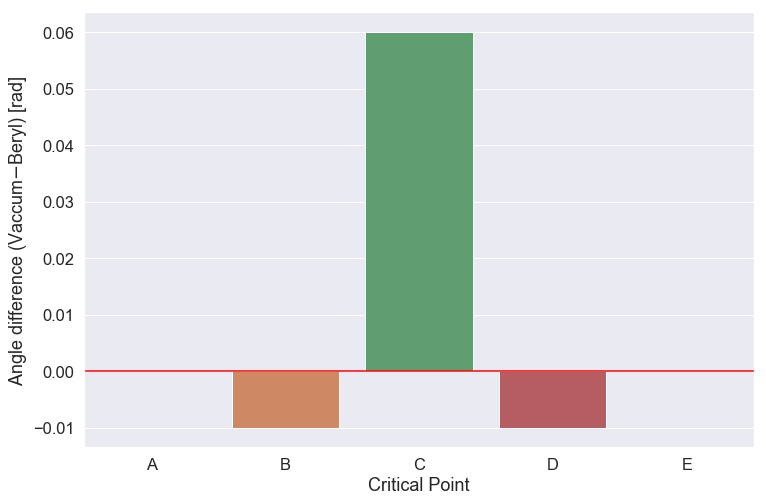
\includegraphics[width=0.9\linewidth]{Figures/System/cp_diff.png}
            \caption{The difference of angles at which the critical points occur. Here, a negative (positive) value indicates that including the framework shifts the critical point to the right (left).}
            \label{fig:cp_diff}
        \end{figure}
        
        The second avenue of investigation provides greater quantitative insight into this static, background potential. By taking the difference in energy between the beryl potential map and the vacuum potential map (with beryl-geometry water molecules), the energy contribution due to the dipole-framework interactions can be determined---this is shown in Fig. \ref{fig:framework_contrubtion}. The results are consistent with those arrived at by examining the critical point shift. That is, the crystal provides a sinusoidal-like increase in energy as the rotation angle increases. Furthermore, since this map is slightly more than half of a sixth of a full rotation, this potential has a six-fold degeneracy, consistent with the symmetry of the crystal. 
        
        \begin{figure}
            \centering
            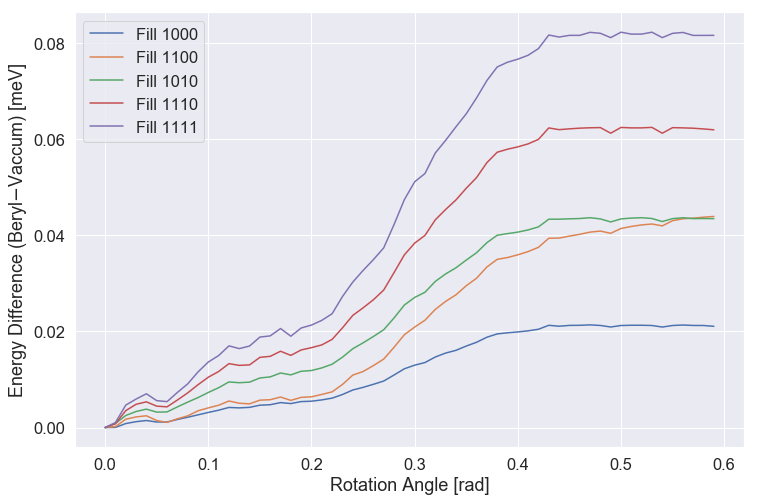
\includegraphics[width=0.9\linewidth]{Figures/System/diff_analysis.png}
            \caption{The difference in potential maps between the beryl and vacuum cases. For consistency, the beryl-geometry water molcules are used for the vacuum case..}
            \label{fig:framework_contrubtion}
        \end{figure}
        
        Also apparent from Fig. \ref{fig:framework_contrubtion} is the fact that fill is not the only relevant parameter for determining the dipole-framework interaction. As evident by the difference in the degenerate $\phi = 0.5$ cases, the specific placement of water molecules is also important. With hopes of trying to find a general relationship, say energy contribution per water molecule, the dipole-framework maps are scaled by the total number of water molecules.
        
        \begin{figure}
            \centering
            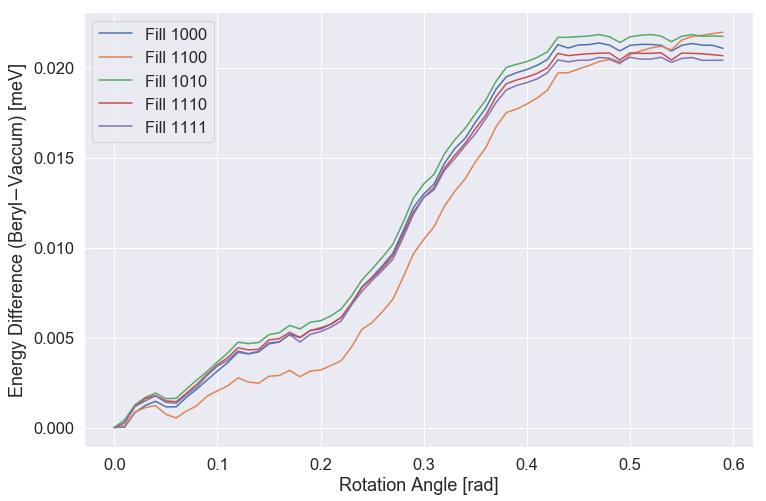
\includegraphics[width=0.9\linewidth]{Figures/System/framework_contribution_scaled.png}
            \caption{The dipole-framework potential maps from Fig. \ref{fig:framework_contrubtion} with the energy scaled by the total number of water molecules.}
            \label{fig:framework_contribution_scaled}
        \end{figure}
        
        Figure \ref{fig:framework_contribution_scaled} shows that the scaled dipole-framework potential maps are beginning to resemble some type of general principle. There is still, however, discrepancies between the individual potential maps, not only between fill types but also degenerate fills as well. This suggests that higher-order dipole-dipole (or even dipole-framework) interactions are relevant. 
        
        Nevertheless, an approximate, general relation can be found by taking the average energy at each rotation angle, as shown in Fig. \ref{fig:framework_contribution_fit}. Here, the error bars represent the standard error of the mean, and a well-defined average energy contribution per water molecule is apparent. Such a feature suggests that a parameterized force-field may be possible in which the framework crystal is coarse-grained away in favor of a rotation-based potential. 
        
        \begin{figure}
            \centering
            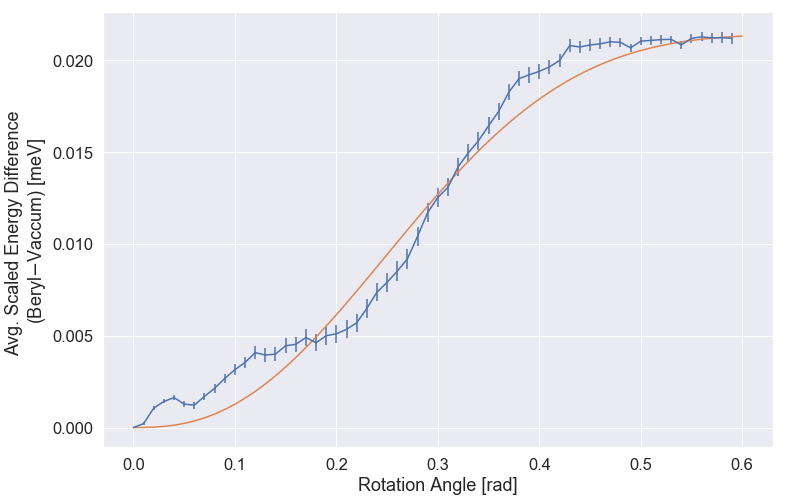
\includegraphics[width=0.9\linewidth]{Figures/System/diff_analysis_fit.png}
            \caption{The average, scaled dipole-framework energy contribution with example of fit. See text for details.}
            \label{fig:framework_contribution_fit}
        \end{figure}
        
        In order for such an approximation to be useful, an analytic function needs to be found, to which the potential map data can be fit. In Fig. \ref{fig:framework_contribution_fit}, a preliminary analytic function is chosen for the fit, specifically
        
        \begin{equation}
        \label{eq:fit}
            E(\theta) = A\sin\left[\frac{\pi}{2} \sin\left( \omega \theta \right)\right]^n,
        \end{equation}

        \noindent for parameters $A,\omega,n$. Equation (\ref{eq:fit}) was chosen after a casual search of sinusoidal functions that exhibit a squished amplitude, but better equations surely exist. Its use here is meant merely to be heuristic in nature. Even still, the fit is decent and hints that this avenue is worth further investigation. 
        
        Besides using an more appropriate analytic function, utilizing a larger unit cell that allows for greater exploration of the fill (and fill-degeneracy) parameter space would yield a more generally appropriate fit. As discussed previously, however, such a large unit cell is cost prohibitive with the resources available for this investigation. Additionally, sampling a full, or at least larger total rotation, within the framework would help in fitting the frequency of analytic function.
        
    \section{Summary and Outlook}
    
    \paragraph{Summary} The Energy Convergence Test (Section \ref{sec:en_conv_test}) provides insights on a few fronts. From a computation standpoint, the larger energy difference tolerance of $10^{-4}$ eV is acceptable for potential map calculations. From a physical standpoint, the calculated potential map tends to agree more with [\textbf{cite pmap2 paper}] in terms of qualitative shape. That is, a six-fold degenerate local minimum occurs when the dipole is co-linear with a nearest-neighbor dipole. In addition, there is a second six-fold degenerate local minimum that corresponds configuration in which the dipole is co-linear with a next-nearest neighbor dipole. In between these two local minima, a 12-fold generate global minimum between the two configurations which does not appear to correspond to any significant case of dipole-dipole alignment.
    
    The Relative Angle Test (Section \ref{sec:rel_ang_Test}) confirms that antiferroelectrically coupled dipole configurations---that is, dipoles with a relative angle difference of $\pi$ radians---are the most energetically favorable. Furthermore, the average energy dependence on the relative angle between dipoles agrees decently with the heuristic
    
    \begin{equation}
    \label{eq:heur}
        E(\alpha) = A \sin(\omega \alpha),
    \end{equation}
    
    \noindent with $A=-0.88$ meV and $\omega = \pi/6$. Deviations from (\ref{eq:heur}) likely represent higher-order dipole-dipole and/or dipole-framework interactions. For the remainder of the investigation, only antiferroelectrically coupled systems are investigated.
    
    In Section \ref{sec:map_v_fill}, the effect that fill has on the potential energy map is investigated. Five fill cases are investigated $\phi \in \{0.25,0.50,0.75,1.00\}$, with a degeneracy in the case of $\phi = 0.50$. As water molecules are added, a dilation effect can be observed in the potential maps. Specifically, the local maxima increase and local minima decrease with each additional water molecule. There is also a noticeable difference between the degenerate $\phi=0.50$ systems, suggesting that relative position of water molecules also plays a role in the energetics, although less significant compared to the effect of fill. In additional the dilation effect, there is a systematic decrease in energy with each water molecule at the rate of $14.3125$ eV/molecule. The fact that the water molecules seem to prefer closer association, at least energetically, is consistent with everyday experiences of water tending to clump together. 
    
    For purposes of disentangling the dipole-dipole interaction from the dipole-framework interactions, a finer range is identified ($0\le\theta\le0.6$) that preserves all distinguishable features and over which a more accurate potential map can be calculated. The results from the Fine Sweep (Section \ref{sec:fine_sweep}) provide the most quantitative insights into the system's energetics. In the beryl case, five critical points A-E are identified that represent the primary local maxima and minima. By looking at the absolute energy difference between said points as a function of fill, a novel method for experimentally determining fill \textit{pre-}experiment is identified, so long as experiment can resolve the energy differences. Examination of the vacuum potential maps pushes this insight further. Again, five critical points are identified that correspond to qualitatively the same maxima and minima. Quantitatively, however, the critical points differ from their beryl-like counterparts in that there is a degeneracy where one did not previously exist. Specifically, points C, E are energetically degenerate. These results suggest that the dipole-framework interaction contributes a static increase in energy. Additionally, there is a difference in the absolute energy of all data points between the vacuum-geometry and beryl-geometry potential maps---the vacuum-geometry is slightly more favorable.
    
    Finally, the differences in these potential maps is analyzed in Section \ref{sec:diff_anal}. First, the angle at which the critical points occur is compared between the vacuum and beryl cases. Both local maxima (B,D) experience a shift towards a higher angle, while the global minimum (C) experiences a shift to a lower angle when the crystal framework is included. This is consistent with the previous assertion about the dipole-framework contribution from the previous section. This contribution is more exactly investigated by taking the difference between the beryl and vacuum cases. As with the previous Map versus Fill test, there is a systematic increase in energy as the fill increases, as well as a lesser dependency on the relative positions of dipoles. When these potential maps are normalized by the total number of water molecules, a more general dipole-framework contribution per water molecule in the average is observed, suggesting that the beryl crystal could be course-grained away assuming a suitable analytic function could be fit to the averaged energy curve. A preliminary function is chosen to demonstrate proof-of-concept
    
    \begin{equation}
    \label{eq:fit}
        E(\theta) = A\sin\left[\frac{\pi}{2} \sin\left( \omega \theta \right)\right]^n,
    \end{equation}
    
    \noindent with $A=0.0214$, $\omega = 2.1772$, and $n=2.5685$$. 
    
    \paragraph{Outlook}
    
    In general, all improvements to the above-described protocols boil down the computational resources. In additional to testing the convergence with respect to energy difference tolerance, testing convergence with respect to cut-off energy, hybrid functionals, etc. would be helpful in bringing the results more inline with nature. Furthermore, a larger unit cell would go a long way in increasing the accuracy of all aggregate results (e.g. being able to sample more fill types and more fill degeneracies). Such a unit cell would also allow for great disentanglement of the energetics, because other relational parameters can be investigated. As it is, though, these would require almost an order of magnitude increase in computational resources.
    
    It would also be interesting to see if a single one-dimensional channel (i.e. only periodic in the $c$-direction) would exhibit a phase transition. If so, it would serve as an example of how a small background perturbation can push a one-dimensional system to a phase transition.
\chapter{Partial Charge Analysis}
\label{ch:part_char}

Having optimized structures and a quantitative point of comparison (namely, the potential maps), the next piece needed to parameterize a force field is the partial charges on the constituent water molecule atoms. 

Many different methods exist for assigning partial charges to atoms, and a systematic process for deciding which is best for the system at hand is desired. Since it is not known \textit{a priori} what the partial charge distribution should look like for the extra-framework water molecules, known systems are used to benchmark the partial charge analysis techniques under the DFT assumptions made thus far. Specifically, the total dipole for the monomer, dimer, and trimer (collectively, n-mer) water cases are calculated and compared to literature values. 

Once a suitable technique is selected, a similar investigative technique as used in the structural optimization and potential map calculations is employed. That is, partial charge analysis is performed on the vacuum-geometry and beryl-geometry water molecule arrays in vacuum followed by analysis on the framework-inclusive system. 

    \section{Benchmark}
    \label{sec:benchmark}
    
    \paragraph{Overview} As mentioned above, there exists different partial charge analysis techniques, each with their own advantages and disadvantages. Specifically, four different techniques are compared: (1) Bader Charge Analysis [\textbf{CITATION}], (2) DDEC analysis with ChargeMol [\textbf{CITATION}], (3) DDEC6 analysis [\textbf{CITATION}], and (4) centers of Maximally Localized Wannier Functions (MLWF) [\textbf{CITATION}]. 
    
    For each method, the total dipole for each of the n-mer water systems is calculated on a structure optimized under the same assumptions (basis set, functionals, etc.) as used in the rest of the work. For methods 1-3, results were qualitatively in agreement with literature values but varied by up to a factor of two otherwise. It is the latter method, using the centers of MLWF, that proved the most accurate; however, issues of convergence appeared that will be discussed below.
    
    \paragraph{Procedure} As discussed briefly in Section \textbf{THEORY SECTION NUMBER}, determining the partial charge via the MLWF is conceptually trivial. In short, a basis transformation from the Bloch functions to non-unique Wannier functions is performed, and then the spread of said Wannier function is minimized to obtain the unique MLWF. From the MLWF, the center can easily be calculated, and this center can be viewed as the classical location for the negative charge. (See theory section or [\textbf{MLWF review citation}] for a more in-depth explanation.) 
    
    Fortunately, it is possible to compile VASP with the VASP2WANNIER library and use said library as a post-processing step on the self-consistent calculations performed for the potential map analysis. This post-processing produces an input file for the Wannier90 software package [\textbf{citation}], which then calculates the actual Wannier centers. In general, the number of centers is equal to the number of electrons in the system, but since all calculations performed here are not spin-polarized, the number of centers is equal to \textit{half} the number of total electrons. Additionally, pseudopotentials are used in lieu of including core electrons. This results in 8 electrons---and therefore, 4 wannier centers---per water molecule.
    
    Once calculated, the Wannier centers need to be assigned to the proper water molecule. This is accomplished with a simple Python script that utilized the ASE library to find the two closest hydrogen atoms and four closest MLWF centers (including periodic images) for each oxygen atom. Each set of oxygen atom, two hydrogen atoms, and four Wannier centers constitutes a water molecule. Using the position and charge ($+6e, +1e, +1e, -2e, -2e, -2e, -2e$ respectively; for elementary charge $e$) for each element, the molecular and total system dipole can be calculated using the classical, discrete definition
    
    \begin{equation}
    \label{eq:dipole_def}
        \Vec{p} = \sum\limits_{i=1}^{N} q_i \Vec{r}_i,
    \end{equation}
    
    \noindent for sum over $N$ total elements, with charge $q_i$ and position $\Vec{r}_i$ of element $i$. Note, it is actually the magnitude of the total system dipole moment $ p = |\Vec{p}|$ that is of particular interest and will be compared to literature values for this benchmark.
    
        \subsection{Convergence Issue} 
        \label{sec:convergence_issue}
        At this point, it is important to point out a significant source of systematic error within this study. The above procedure should result in reproducible dipole moments. Unfortunately, that is not the case. When running the exact same post-processing procedure on the same self-consistent wavefunction, different dipole moments are calculated. Most of these calculated dipoles fluctuate around the expected values, but outliers that are up to 50 times too large can also appear.
        
        \begin{figure}
            \centering
            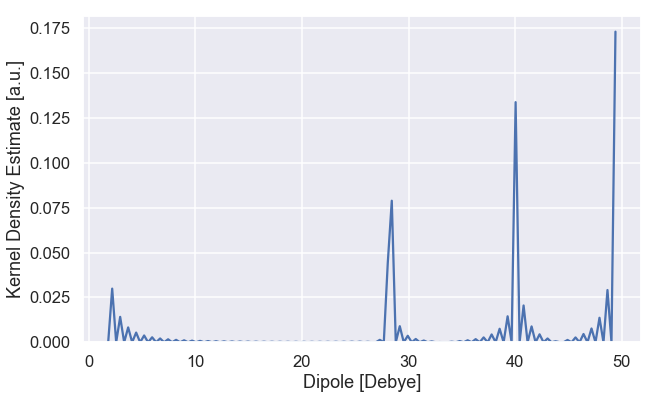
\includegraphics[width=0.9\linewidth]{Figures/System/pc_bad_convergence.png}
            \caption{The Kernel Density Estimate of the total dipole for a sample set of 25 monomer dipole calculations.}
            \label{fig:pc_bad_convergence}
        \end{figure}
        
        Figure \ref{fig:pc_bad_convergence} shows an example of this calculated dipole fluctuations. Here, the same converged wavefunction for a monomer is used to calculate the dipole 25 times, and the kernel density estimate (KDE) for the population is plotted. A peak occurs around the expected value of 1.86 D, but three additional peaks occur for much higher dipole values. (Note, the height of the peak does not necessarily correlate the number of sample with that value and is largely meaningless at this point.) All together, this suggests that some parameter in the system is not well converged.
        
        In an attempt to rectify this issue, a zoo of parameters was put through a tuning process, including: basis set size, $k$-point sampling, box size, number of self-consistent steps, smearing, number of empty bands used in the calculations, and energy difference tolerance. In all cases, similar fluctuations in dipole values resulted. Furthermore, it appears that many people have experienced the exact same issue when attempting to calculated the dipole of a monomer using the VASP and Wannier90 software packages in conjunction with the VASP2WANNIER library [\textbf{mailing list citations}]. 
        
        From reading the identical issues and from personal correspondence with some of the researchers experiencing said issue, the problem likely occurs when the VASP2WANNIER library is called to project the Bloch states on the Wannier states. The only person identified that was able to solve this problem did so by using a different \textit{ab initio} software package [\textbf{cite personal correspondence}]. For sake of consistency and time, however, a different approach is used to overcome this convergence issue.
        
        \paragraph{Removing Outliers} For the n-mer cases, it is trivial to remove the outliers, because there exists an accepted value in literature. However, for the array of water molecules used to calculate the potential maps, no \textit{a priori} value can be found, necessitating a quantitative and systematic way to determine and remove the outliers. This is accomplished via the modified Z-score.
        
        The modified Z-score is an extension of the standard Z-score 
        \begin{equation}
        \label{eq:z_score}
            Z_i = \frac{x_i - \Tilde{x}}{\sigma},
        \end{equation}
        
        \noindent for measurement $x_i$, sample mean $\Tilde{x}$, and sample standard deviation $\sigma$. Essentially, eq. (\ref{eq:z_score}) transforms the datum $x_i$ into units of standard deviations from the sample mean. Using the Z-score on small sample sizes is known to yield misleading results for small sample sizes [\textbf{citation}].
        
        Rather than use the sample mean, the modified Z-score uses the more robust median value, since it is less sensitive to large outlier fluctuations. This score is defined as
        
        \begin{equation}
            M_i = \frac{x_i - \Bar{x}}{\mu},
        \end{equation}
        
        \noindent for sample median $\Bar{x}$ and median absolute deviation $\mu$ [\textbf{citation}]. Rejecting the outliers becomes a simple task of tuning a tolerance $s$, for which a modified Z-score that is greater $M_i>s$ identifies an outlier. Note, a smaller $s$ value corresponds to being more discriminatory towards outliers.
        
        
        
        \begin{figure}
            \centering
            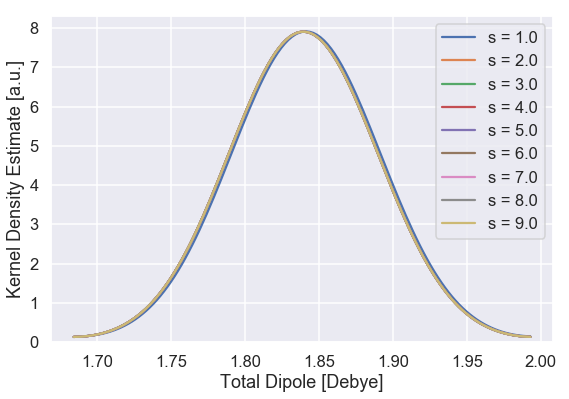
\includegraphics[width=0.3\linewidth]{Figures/System/pc_m_scan_monomer.png}\hfill
            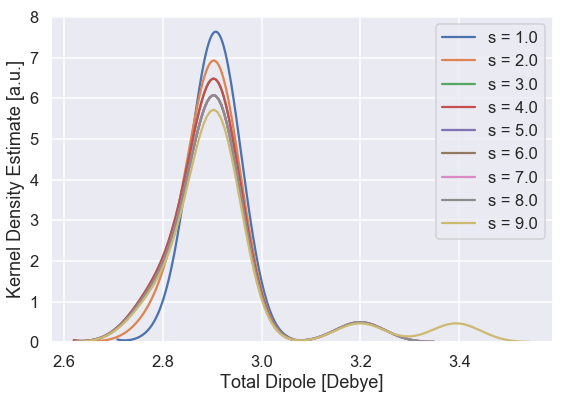
\includegraphics[width=0.3\linewidth]{Figures/System/pc_m_scan_dimer.png}\hfill
            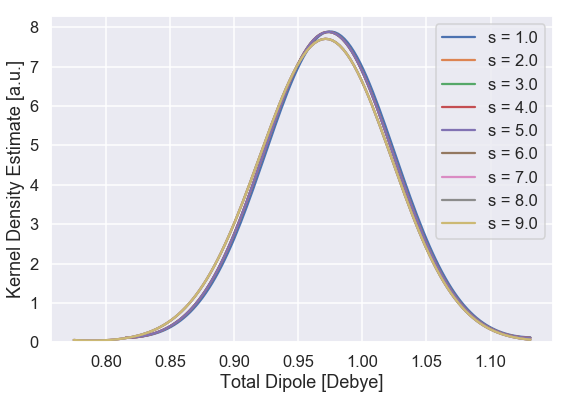
\includegraphics[width=0.3\linewidth]{Figures/System/pc_m_scan_trimer.png}\hfill
            \caption{Tuning results for the modified Z-score tolerance $s$. (Left) Monomer, (center) dimer, (right) trimer.}
            \label{fig:m_scan}
        \end{figure}
        
        Figure \ref{fig:m_scan} shows the monomer, dimer, and trimer total dipole KDEs (left, center, and right therein) for different tolerance values $s$. As seen in all three cases, a well-defined peak is visible. In the case of the monomer and trimer, there appears to be little sensitivity to tolerances over the range investigated. For the dimer, larger dipole peaks appear for the larger tolerance (less discriminatory) values. These vanish for $s<6$, and the peak is maximized for $s=1$. Therefore, for sake of consistency, $s=1$ is used for all outlier rejections throughout.
        
        One more note on the outlier removal procedure. Generally, there are two different data sets of dipole values on which one could detect outliers---the individual dipoles and the total system dipole. In order to maximize the signal-to-noise ratio, the modified Z-score should be calculated on the total dipole for each configuration, and if it is determined to be an outlier, \textit{all} of the individual dipoles that correspond to that configuration should be discarded. The underlying assumption being that if the total dipole is an outlier, then the calculation was not well-converged and the individual dipole measurements are not reliable.
        
        \begin{figure}
            \centering
            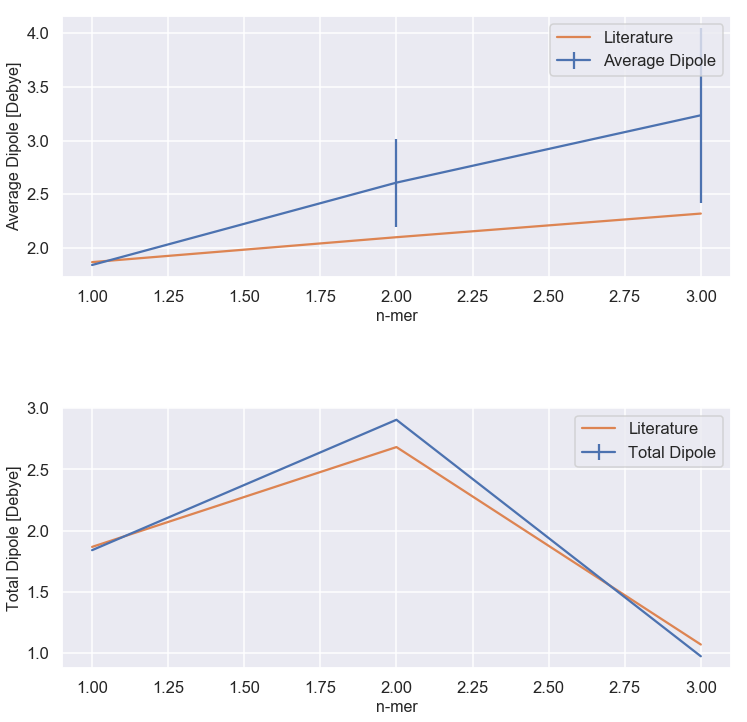
\includegraphics[width=0.9\linewidth]{Figures/System/pc_benchmark_results.png}
            \caption{Results for the n-mer partial charge benchmark. (Top) Average individual dipole; (bottom) total system dipole.}
            \label{fig:pc_bench_results}
        \end{figure}
        
        \subsection{Results and Analysis} The results for the n-mer partial charge benchmark using the above described Wannierization, charge assignment, and outlier removal are compared to literature results [\textbf{n-mer citation}] in Fig. \ref{fig:pc_bench_results}. Here, error bars represent the standard error of the mean and are not visible within the resolution of the bottom graph. Clearly, the results are in good qualitative and quantitative agreement with the literature values. Discrepancies between the two are attributed to the use of differently optimized structures, different basis sets, and different functionals. 
        
        As such, the above described procedures are deemed appropriate to use in order to perform partial charge analysis on the beryl and vacuum systems.
        
    \section{Extra-Framework Water Analysis}
    
    Having established the efficacy of the proposed partial charge analysis method, the average dipole as a function of fill, rotation, and local environment are investigated. However, first a resource-imposed limitation is highlighted.
    
    The cost for collecting a large enough sample size to perform any meaningful dipole of statistical analysis on the water molecule dipoles is quite high. In the case of the benchmark, 25 runs for each system were calculated, with a nearly 50\% rejection rate. For the actual system under investigation, there exists 60 different configurations for each fill type, and each one of those requires multiple runs. For the vacuum case, it is feasible to do the same number of runs (i.e. 25) as the benchmark, with run times of about 12-14 days. For the beryl case, there exist nearly 20 times as many ions and electrons, and only ten runs per configuration can be run in the same amount of time. 
    
    Therefore, vacuum case results are prioritized for both the vacuum-geometry and beryl-geometry water molecules. Data for the beryl cases will be collected up until point of submission, and the results attained will also be reported below.
    
        \subsection{Vacuum Case}
        \label{sec:pc_vacuum_Case}
        
        \textbf{Procedure} As mentioned above, the relatively small system size for the vacuum case allows for a larger sample size to be collected. Specifically, for both the vacuum-geometry and beryl-geometry water molecules, the individual and total dipoles are calculated according to the benchmark procedure 25 times for each self-consistent configuration calculated during the potential map investigation. Outliers rejection tolerance is set to $s=1$.
        
        \textbf{Results and Analysis} Figure \ref{fig:pc_vacuum_kde} gives the KDEs for the individual dipoles for both the vacuum- and beryl-geometry water molecules (left and right, respectively therein) as a function of fill and for all configurations. For the vacuum-geometry case, the results for fill 1000 are omitted for ease of reading, but an almost $\delta$-function-like peak occurs for $p = 1.96$ D. While a quantitative comparison is not discernible from this figure, it is clear that describing the dipole data sets in an average manner is appropriate.
        
        \begin{figure}
            \centering
            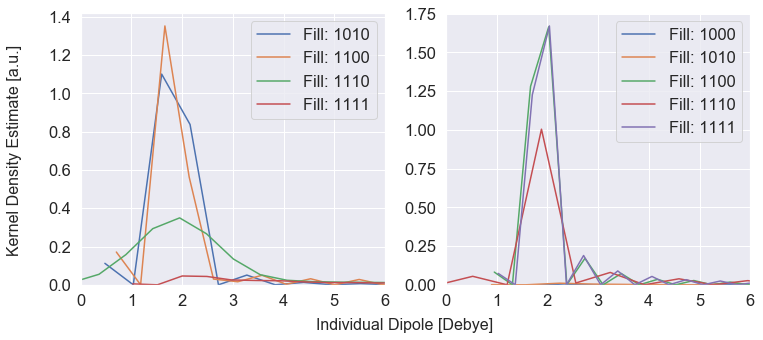
\includegraphics[width=0.9\linewidth]{Figures/System/pc_vacuum_compare_kde.png}
            \caption{The individual dipole KDEs by fill for the vacuum- (left) and beryl-geometry (right) water molecules in vacuum. Note, for the vacuum-geometry case, the results for the 1000 fill case are omitted for clarity.}
            \label{fig:pc_vacuum_kde}
        \end{figure}
            
        The average individual dipole as function of fill for water molecules with both the vacuum-geometry (solid, blue line) and beryl-geometry (dashed, black line) is shown in Fig. \ref{fig:pc_vacuum_avg_dipole}. In general, the qualitative behavior of the dipole as a function of fill does not change drastically with respect to geometry, which is as expected. The main difference appears to be a contraction effect of the dipole when moving from the vacuum- to beryl-geometry water molecules. These results are consistent with the structural optimization results found in Section \ref{sec:geom_opt}. Namely, the framework has a dilating effect on the water geometry, with both the blond length $r$ and OHO angle $\theta$ increasing (the latter being more significantly increased than the former). 
        
        If the water molecule is thought of being positioned as in Fig. \ref{fig:pc_analysis}, the individual dipole is along the $+x$-direction, and the magnitude $p$ is proportion to the projection of $r$ on the $x$-axis. That is, 
        
        \begin{equation}
            p \propto r \cos\left(\frac{\theta}{2}\right).
        \end{equation}
        
        \noindent Since the percent difference between the 25\% and 100\% fill is greatest for the OHO angle $\theta$ (approximately 1.1\% compared to 0.1\% for the bond length $r$), the bond length can be thought of as being nearly constant. Therefore, as the angle $\theta$ increases, the projection onto the axis decreases---and so goes the dipole magnitude.
        
        \begin{figure}
            \centering
            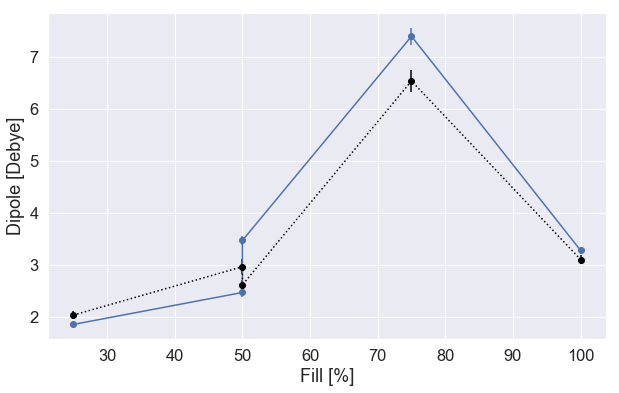
\includegraphics[width=0.9\linewidth]{Figures/System/pc_vacuum_avg_dipole.png}
            \caption{The average individual water molecule dipole as a function of fill. Again, the solid, colored line represents vacuum-geometry results, while the dashed, black line represents beryl-geometry results. Error bars represent the standard error of the mean.}
            \label{fig:pc_vacuum_avg_dipole}
        \end{figure}
        
        The contraction-inducing influence on the dipole moment does not universally result in an increase or decrease in dipole moment, as shown in Fig. \ref{fig:pc_vacuum_dipole_ratios}. Here, the average individual dipole moment ratio between the vacuum- and beryl-geometry water molecules is given as a function of fill. The red line indicates unity, and therefore, ratios below (above) unity indicate a(n) decrease (increase) in the dipole moment when moving from the vacuum- to beryl-geometry. A decrease is observed for fill 25\%, and an increase is observed for the remaining fills. 
        
        \begin{figure}
            \centering
            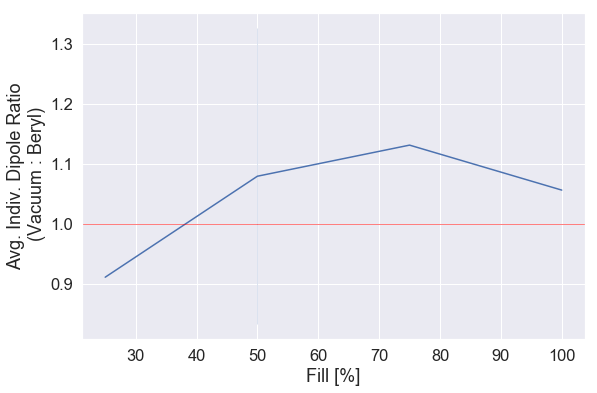
\includegraphics[width=0.9\linewidth]{Figures/System/pc_vacuum_dipole_ratios.png}
            \caption{The ratio of the individual dipole (vacuum- to beryl-geometry} as a function of fill. The red line denotes unity.
            \label{fig:pc_vacuum_dipole_ratios}
        \end{figure}
        
            \subsection{Partial Charge Assignment}
            \label{sec:pc_assign}
            
            Using the dipole results in conjunction with the structural optimization results, the partial charges are assigned using the following procedure.
            
            \begin{figure}
                \centering
                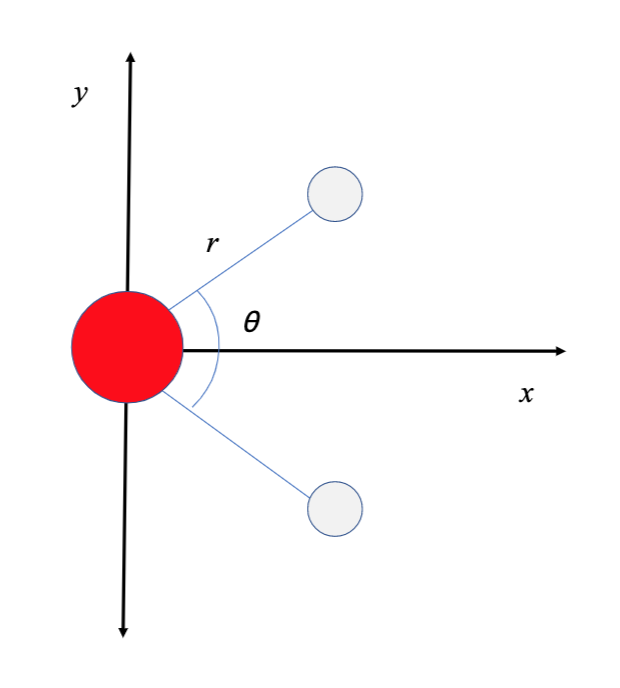
\includegraphics[width=0.5\linewidth]{Figures/System/pc_analysis.png}
                \caption{Diagram of a model molecule in the $xy$-plane with the oxygen atom centered at the origin. See text for details.}
                \label{fig:pc_analysis}
            \end{figure}
            
            \paragraph{Procedure} Consider first a water molecule in the $xy$-plane, with the oxygen atom at the origin and hydrogen atoms at $(r\cos\alpha,\pm r\sin\alpha)$ with $\alpha = \theta/2$, as shown in Fig. \ref{fig:pc_analysis}. The dipole magnitude is given by
            
            \begin{equation}
            \label{eq:dip_mag}
                p = 2n_H|e| r \cos\left(\frac{\theta}{2} \right)\hat{x},
            \end{equation}

        \noindent for hydrogen atom partial charge assignment $n_H > 0$ and elementary charge $e$. From (\ref{eq:dip_mag}), the partial charge assignment for the oxygen and hydrogen atoms are given, respectively, as
        
        \begin{eqnarray}
        \label{eq:pc_assign}
            n_H &=& \frac{p}{2er} \sec\left( \frac{\theta}{2} \right)  \\
            n_O &=& -2n_H 
        \end{eqnarray}
        
        \paragraph{Results and Analysis} The partial charge assignment for the oxygen atom is given as a function of fill in Fig. \ref{fig:pc_vacuum_pc}. In qualitative terms, the results are equivalent to the dipole results in Fig. \ref{fig:pc_vacuum_avg_dipole}, although here in the negative since oxygen is electronegative. A distinct feature is apparent for the 100\% fill case, however, in that the partial charge assignment appears to be close to identical. In fact, systematically the difference between the geometry cases appears to be indirectly proportional to fill, with the except of the degenerate 50\% cases, wherein the partial charge also appears to be nearly identical.
        
        \begin{figure}
            \centering
            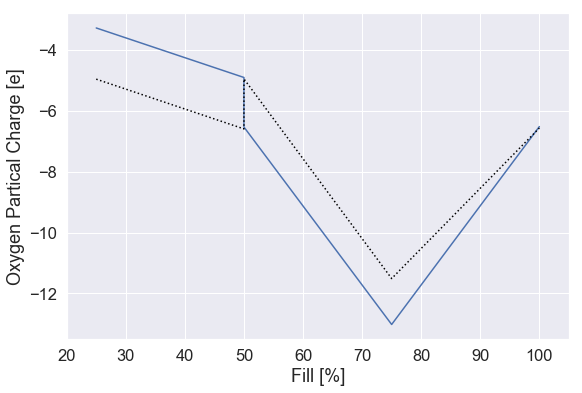
\includegraphics[width=0.9\linewidth]{Figures/System/pc_vacuum_pc.png}
            \caption{The oxygen partial charge assignment as a function of fill for the vacuum- (solid,blue line) and beryl-geometry (dotted, black line) water molecules.}
            \label{fig:pc_vacuum_pc}
        \end{figure}
        
        These observations are explored deeper with the help of Fig. \ref{fig:pc_vacuum_pc_ratios}. Here, the ratios of the vacuum- to beryl-geometry oxygen partial charge assignment are given as a function of fill. The red line indicated unity. Again, the qualitative behavior here is similar to that in Fig. \ref{fig:pc_vacuum_dipole_ratios}, and the fill 50\% and fill 100\% cases are closest to unity. The minimally filled case represents the greatest discrepancy between the two geometry cases.
        
        \begin{figure}
            \centering
            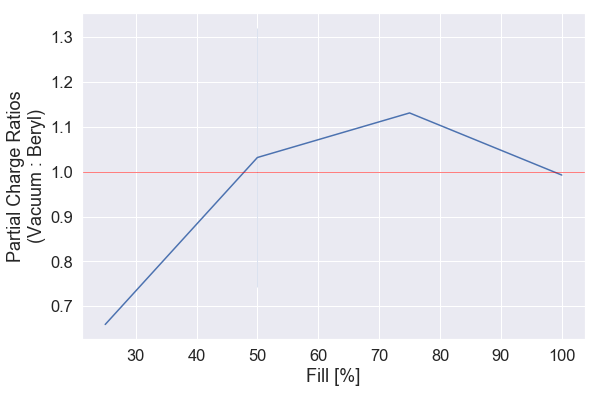
\includegraphics[width=0.9\linewidth]{Figures/System/pc_vacuum_pc_ratios.png}
            \caption{Oxygen partial charges ratios between the vacuum- and beryl-geometry cases as a function of fill. The red line indicated unity.}
            \label{fig:pc_vacuum_pc_ratios}
        \end{figure}
        
        
        \subsection{Beryl Case}
        \label{sec:pc_beryl_case}
        
        As mentioned before, determining the MLWF centers, and hence the partial charge, for the water molecules in the beryl framework is quite expensive. In the same amount of time that the vacuum case calculations can be made 25 times per configuration, only ten in-framework calculations per configuration can be performed. Due to time limitations, it is unclear if all of the fills will be investigated before completion of this work, but what results are attained are reported below.
        
        \paragraph{Procedure} The same procedures as utilized in the vacuum cases are used for both the generation of the Wannier data and the partial charge assignment. As noted, however, only ten Wannier calculations are performed for each configuration.
        
        \paragraph{Results and Analysis} The preliminary results for the average individual dipole for water molecules in the beryl framework (blue circle) are given in Fig. \ref{fig:pc_beryl_pc}. For comparison, the results for vacuum cases with beryl- and vacuum-geometry (orange and green dots, respectively) are provided for comparison. On average, the dipole moment for the water molecule in beryl is slightly smaller than its in-vacuum counterpart. However, both cases are indistinguishable from each other when considering the error. Whether or not they would remain indistinguishable as better statistics are achieved is uncertain, but the prospect hints at a more efficient way of calculating the dipoles. Namely, use the in-framework geometry in the vacuum case---saving potentially weeks of calculations. Also, if this indistinguishability holds, it would support the idea that the framework interacts nominally with the dipole-dipole system.
        
        \begin{figure}
            \centering
            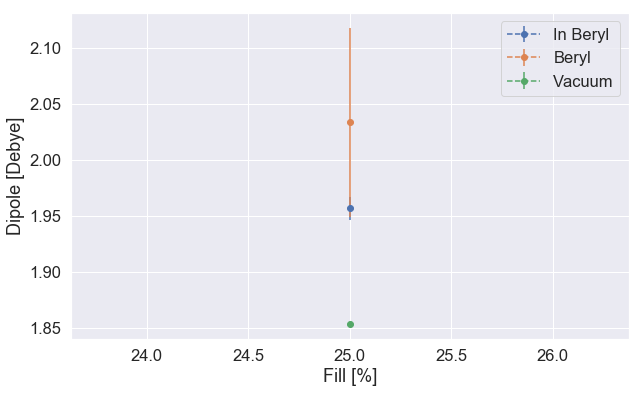
\includegraphics[width=0.9\linewidth]{Figures/System/pc_beryl_pc.png}
            \caption{The average individual dipole moment as a function of fill for extra-framework water molecules in the beryl framework (red). The vacuum cases with vacuum- and beryl-geometry (green and blue, respectively) are provided for comparison.}
            \label{fig:pc_beryl_pc}
        \end{figure}
        
        The discrepancy between partial charge is even less than that for the dipole, with the in-framework and beryl-geometry vacuum cases agreeing to six decimal places (a few orders of magnitude greater accuracy than this study is claiming) for the oxygen atom partial charge
        
        \begin{equation}
            q_O = -4.947902\text{ } |e|.
        \end{equation}
        
    \section{Summary and Outlook}
    
    Overall, the partial charge analysis stage proves to be the biggest bottleneck in terms of computational resources needed. As discussed in Section \ref{sec:benchmark}, this is because of a known convergence issues in the Wannierization procedure using VASP, Wannier90, and the VASP2WANNIER library. Even still, a workable procedure that involves rejecting outliers using the modified Z-score is identified and used to benchmark the cases of the water monomer, dimer, and trimer (Section \ref{sec:convergence_issue}). The results for both individual dipole and total dipole generally agree with the results found in literature, providing confidence in the prescribed procedure.
    
    Overcoming this convergence issue should be a primary focus for future studies, and said studies would be advised to use the water n-mer cases as a benchmark when choosing functionals, basis sets, etc. Also, other partial charge analysis methods (e.g. DDEC6) may yield better results under different approximations. If such a set of approximations can be found, using DDEC6, for example, would results in orders of magnitude decrease in the cost of this step.
    
    Next, the vacuum case for extra-framework water molecules---both with vacuum- and beryl-geometry---is examined in Section \ref{sec:pc_vacuum_Case}. Both geometry cases exhibit similar dipoles as function of fill, but the beryl-geometry case experiences a \textit{contraction}-like effect that is consistent with the \textit{dilation}-like effect on geometry found previously. As mentioned numerous times before, examining larger unit cells with greater fill degeneracy would be of particular interest, because it would allow for a more general dipole versus fill curve to be found.
    
    A procedure for using the optimized geometry results and dipole results to determine the partial charge assignments in outlined in Section \ref{sec:pc_assign}. The resulting oxygen partial charge assignments mirror the dipole results in the sense that the differences between the two geometry cases are qualitatively negligible. For the partial charge; however, there is less discrepancy in partial charge assignment between the two geometry types than the dipole magnitudes.
    
    Finally, preliminary results for the case of extra-framework water molecules in the beryl crystal are provided in Section \ref{sec:pc_beryl_case}. As discussed, these calculations are significantly more expensive than the vacuum counterparts, and only a partial data set is available as of time of writing. From the available results, it appears that very little difference in dipole magnitude, and even less difference in partial charge assignment, exists between the beryl-geometry in vacuum and the in-beryl cases. If this trend holds as more data is attained, it would suggest a significant increase in productivity by allowing for partial charge assignment to be calculated in-vacuum. Having the dipole-framework contribution parameters as degrees-of-freedom also makes this approach more plausible.

\chapter{Summary and Conclusions}
\label{chap:conclusions}


The work presented not only elucidates the structural and electronic properties of nanoconfined water molecules in beryl, but it also identifies a computational protocol for studying similar crystal systems. The top-line conclusions and outlook for each portion of the study are presented below followed by the proposed computational protocol.

\section{Structural Optimization} 

\paragraph{Equation of State Fitting} First in Chapter \ref{ch:struct_opt}, the Birch-Murnaghan equation of state for the beryl framework was sampled and fit, and an equilibrium volume of $V_0= 695.39$ $\angstrom^3$ and bulk modulus of $B_0 = 1.1249$ eV/$\angstrom^3$ was found. These values are in good agreement with literature values \textemdash  $V_\text{lit} = 675\pm0.1$ $\angstrom^3$ and $B_\text{lit} = 1.1\pm0.01$ eV/$\angstrom^3$ \textemdash especially considering the latter where found at ambient conditions, and the former were calculated at zero temperature. 

\paragraph{Decoupling Assumption} Within the equilibrium structure, the assumption stating that the framework and extra-framework dynamics can be decoupled was confirmed by relaxing the ionic positions two ways: (a) allowing all ions to relax and (b) allowing only the water ions to relax. (These two methods are referred to as the full and selective relaxations, respectively.) Additionally, convergence of the ionic positions was also tested for two energy stopping tolerances EDIFF = $10^{-4},10^{-6}$. No measurable difference of significance was found between the full and selective relaxation schemes. Furthermore, the structural parameters were found to be well-converged with respect to the larger EDIFF values. Therefore, the selective relaxation scheme with the larger energy stopping tolerance are deemed acceptable for the geometry optimization.

\paragraph{Geometry Optimization} Different arrangements of water molecules were allowed to relax under the selective relaxation scheme with a variety of fills and relative angles. The same relaxations were also carried out without the beryl framework atoms (i.e. in vacuum) so that the influence of the framework itself could also be determined. For each fill factor, the geometry parameter distribution with respect to relative angles between water molecule is such that it is meaningful to describe the parameters using average values. Furthermore, there was a measurable difference between both the fill factor geometries and those with/without the beryl framework. The numeric results are provided in Table \ref{tab:geo_sum}. In general, the bond length is directly proportional to the fill, while the angle is indirectly proportional; and the beryl framework has a global dilation effect on the water molecules. That is, the presence of the beryl framework causes a systematic increase in both the bond length and the angle.

\begin{table}[]
    \centering
    \begin{tabular}{c|c|c}
      Fill & Bond Length [$\angstrom$] & Angle [deg] \\
      \hline
      \hline
      0.25   & 0.97298(29)    & 105.35(08) \\
             & [0.97214(08)]  & [104.40(49)] \\
     \hline
      0.50   & 0.97294(40)    & 105.19(12) \\
             & [0.97219(50)]  & [104.36(14)] \\
     \hline
      0.75   & 0.97313(39)    & 105.09(13) \\
             & [0.97228(68)]  & [104.18(26)] \\
     \hline
      1.00   & 0.97322(64)    & 104.81(25) \\
             & [0.97252(86)   & [104.16(24)]
    \end{tabular}
    \caption{The geometry parameters as a function of fill. The values in square brackets denote parameters calculated in vacuum. The values in parenthesis represent the error. For the bond length the error is given in $\micro\angstrom$, and for the angle, the error is given in 0.001$^{o}$. }
    \label{tab:geo_sum}
\end{table}

One possible improvement identified for this protocol involves the configurations used to sample the geometries. All geometries were sampled at symmetry points within the crystal. It may be worthwhile to perform the relaxation with randomly chosen water molecule positions, both relative to the framework and other extra-framework water molecules.

\section{Potential Maps}

\paragraph{Broad Sweep} To determine the smallest range through which water molecules can be rotated and still recover all significant features of the potential map at the high-symmetry point, two ferroelectrically coupled water molecules with fill 1010 are rotated through $\pi$ radians. As with the geometry relaxation, the convergence of the energy is tested with respect to EDIFF; except here, energy stopping tolerance of $10^{-4}$ and $10^{-6}$ are tested. Two local minima, corresponding to configurations with water molecule dipoles being co-linear with nearest and next-nearest neighbor dipoles, are identified that both have six-fold degeneracy. An additional 12-fold degenerate global minimum exists in between said local minima, but it is not clear whether or not this corresponds to any significant arrangement. These results confirm and extend the potential map assumptions used in previous studies. Additionally, no significant difference in the potential maps was found with respect to the two energy stopping tolerances.

It is concluded that a smaller rotation range of $\pi/2$ radians with the larger energy stopping tolerance of $10^{-4}$ is appropriate for the remaining potential map calculations.

\paragraph{Relative Angle Test} Next, the ferroelectric coupling is lifted, and potential maps are calculated with various relative angles between the two water molecules. As expected, the antiferroelectric alignment minimizes the energy of the potential maps systematically. Furthermore, when disregarding the angle relative to the beryl crystal, the potential energy as a function of relative angle between water molecules closely follows the heuristic of two classical dipoles interacting, with deviations being attributed to high-order dipole-dipole, or even dipole-framework, interactions. 

\paragraph{Map vs. Fill} Using the antiferroelectric coupling moving forward, the potential maps are calculated as a function of fill. It is found that with each additional extra-framework water molecules, the potential energy decreases on average by 14.3125 eV. This suggests that the system prefers to be completely filled with water molecules, at least from an energetics standpoint. 

In an attempt to disentangle the dipole-framework and dipole-dipole interactions, fine sweep potential maps are carried out over a slightly smaller rotation range (0.6 radians) with a larger sample frequency for the extra-framework water molecules rotating in beryl and in vacuum.

\paragraph{Fine Sweep} Beginning with the in-beryl case, five critical points A-E are identified, correspond to local minima (A,C,E) and local maxima (B,D). By comparing the difference in energy between these critical points as a function of fill, a linear dependence on fill is found. Assuming such energy differences could be resolved in experiment, this feature may provide a way to experimentally determine the fill of a sample \textit{before} optical experiments are performed, rather than after, if a reference curve can be experimentally fit. 

Next, the in-vacuum potential maps are calculated as a function of fill in two ways: (a) with the vacuum-geometry water molecules and (b) with the beryl-geometry water molecules. In both cases, the qualitative features of the potential maps remain, suggesting that features result primary due to the dipole-dipole interactions. There is a slight energetic preference for the vacuum-geometry water molecules, but the difference in negligible when compared to the energy difference due to fill. Again, the energy difference of the five critical points (A-E) are analyzed, but this time, a degeneracy is found between the local minima C and E. Therefore, in the absence of the framework, the dipole-dipole system experiences a six-fold degenerate local minimum an 18-fold degenerate global minimum. 

By comparing the in-beryl and in-vacuum cases, it appears that the beryl framework contributes a slight pertubation that lifts the global minimum degeneracy. This observation is explicitly tested in the next subsection. 

\paragraph{Difference Analysis} By subtracting the in-vacuum potential maps (with beryl-geometry water molecules) from the corresponding in-beryl potential maps, the energetic contributions from the dipole-framework interactions is analyzed. It is found that the framework contributes a sinusoidal-like background potential for the dipole-dipole system. This background potential can be scaled by the total number of water molecules to yield a per-molecule background potential. By taking the average of these per-molecule background potentials over fill, a well-mannered master per-molecule background potential is found. 

The existence of such a master background potential suggests that if it can be fit to an analytic function, future potential maps could be calculated without the framework atoms, significantly reducing the computational cost. This reduction in computational cost would allow for one of the greatest improvements of this work to be implemented \textemdash specifically, using a larger unit cell, which would allow for more fill factors, and more degenerate configurations for each fill factor, to be investigated. This improvement is desired, because slight differences between the degenerate fill 0.50 cases were seen. While these differences were negligible compared to the effects of fill itself, they suggest that the spatial arrangement of the water molecules also affects the energetic of the system. Hence, a larger unit cell would allow for a greater exploration of this parameter space.

\section{Partial Charge Analysis}

\paragraph{Benchmark} The partial charge analysis contains the greatest amount of systematic error. Although the Wannierization proves to be the most consistent for the cases of the n-mers dipole moments, an issue with convergence is apparent in the lack of reproducible dipole calculation results. This issue is not unique to this work, and others have posited that there is a poorly converged position operator in the Wannierization process. This poor convergence causes the Wannier centers, and therefore the dipole moments, to fluctuate around the expected value; however, some of these fluctuations result is very large, unexpected dipole moments. 

Since the expected results are known for the n-mer cases, sample sets were collected for each case. A modified Z-test was then tuned to detect and remove the outliers. With confidence in the methodology established by decent results for the n-mer cases, this protocol was followed for partial charge analysis.

\paragraph{Extra-Framework Water Analysis} Partial charge analysis was carried out for the vacuum case (with both water-molecule geometries) and the beryl case. For the vacuum cases, the results are consistent qualitatively with respect to geometry. This further bolsters confidence in the applied technique. The average dipole moment per molecule is proportional to the fill, but a sharp increase in the dipole moment is observed for fill factor $\phi=0.75$. It is not clear form the data set why this case should have such a high dipole moment, but the differences in the degenerate $\phi =0.50$ offer a clue. It appears that the dipole moment is much more sensitive to the relative position of extra-framework atoms than the energy or the geometry. Perhaps if a larger unit cell were used with more degenerate cases, the $\phi=0.75$ results would appear less dramatic.

Results are only available for a portion of the beryl-case fills due to the high computational cost of acquisition \textemdash approximately four weeks per fill. From the $\phi=0.25$ case, there appears to be a slight decrease in the average dipole moment compared to the beryl-geometry vacuum case, but when the error bars are considered, the results are indistinguishable. If this consistency holds with the other fills, or more convincingly with better statistics for the vacuum case, removing the framework atoms for purposes of calculating partial charges would offer orders of magnitude increase in efficiency.

The numerical results for all available partial charge assignments are given in Table \ref{tab:partial_charge}.

\begin{table}[]
    \centering
    \begin{tabular}{c|c|c|c}
       Fill  & Vacuum$^{1}$ & Vacuum$^2$ & Beryl   \\
       \hline
       \hline
       1000  & -3.26 &  -4.95 & -3.32 \\
       1010  & -4.89 &  -4.94 & \textemdash  \\
       1100  & -6.52 &  -6.59 & \textemdash \\
       1110  & -13.02 & -11.51 & \textemdash \\
       1111  & -6.51 &  -6.56 & \textemdash \\
    \end{tabular}
    \caption{Partial charge assignments in units of elementary charge $e$ for the oxygen ions. $^1$Vacuum case with vacuum-geometry water molecules. $^2$Vacuum case with beryl-geometry water molecules}
    \label{tab:partial_charge}
\end{table}

Either resolving the convergence issue, collecting larger data sets, or utilizing a more sophisticated outlier technique would all likely provide the most significant improvement in the confidence of these results. Potential untested culprits for the convergence issue are basis set and functional. Collecting a larger data set, especially for the potential map cases, will require weeks to months worth of computational time on the JUSTUS cluster. There may exist methods for outlier detection that also take into account the dipole measurements of other systems, perhaps in the realm of machine learning.

\section{Computational Protocol}

Based upon the experience gained during the course of this work, the following protocol is proposed for future studies. 

\paragraph{Benchmark} Seeing as the partial change assignments are the least-converged quantity, all parameter choices should be benchmarked against the n-mer dipole moments rather than the energy or structural parameters.

\paragraph{Structural Optimization} Begin by sampling and fitting the equation of state curve. A more accurate description may be achievable by fitting to multiple equations of state and aggregating the results. Once the crystal framework has been optimized, begin relaxing water molecules over a multitude of fill and rotation configurations. Choosing said configurations stochastically may provide improvements over the results in this study. 

\paragraph{Potential Maps} If only interested in groundstate properties, calculating the potential maps with antiferroelectrically coupled water molecules is appropriate.

\paragraph{Partial Charge Assignment} Finally, using the self-consistent wavefunctions from the potential maps, perform Wannierization to obtain the Wannier function centers. Using the resulting dipole moment and water molecule geometry, calculate the partial charge assignment.

\section{General Outlook}

One open question is whether or not a classical force field can be parameterized that produces the same groundstate potential map. While initial guesses for the physical parameters is obtained from this work, choices for the computational parameters (Lennard-Jones coefficients, cut-offs, etc.) are not. While the van der Waals interactions are thought to be weak, attempting to determine an initial guess from DFT methods would be an ideal first step. Then, different cut-offs for the Coulomb interaction can be investigated. Since the most significant features appear to arise from dipole-dipole interactions, it is not clear how large this value should be. Tuning this parameter against the DFT potential maps would help elucidate how many \textit{neighbors} significantly interact with each water molecule.

Another step in parameterizing a force field would be fitting the framework contribution to an analytic function. While not necessarily conceptually challenging, this will require comparing a lot of candidate equations.

Since the framework contribution lifts an energy degeneracy in the global minimum, it would also be interesting to see if a one-dimension chain of water molecules in the beryl framework exhibit a phase transition. Whether or not the production of such systems would be technically possible is unknown.

Exploring all of the above as a function of pressure would also be of interest and is in-line with current experimental work.

Overall, it is clear that these systems and avenues of research are ripe with questions and worthy of future research.


\appendix
%%%%%%%%%%%%%%%%%%%%%%%%%%%%%%%%%%%%%%%%%%%%%%%%%%%%%%%%%%%%%%%%%%%%%%%%%%%%%%%%%
%2345678901234567890123456789012345678901234567890123456789012345678901234567890
%        1         2         3         4         5         6         7         8
% THESIS APPENDIX

\chapter{Gesture Vocabulary} 
\label{chap:appendixA}


\begin{figure}
    \centering
    \includegraphics[width=0.8\textwidth]{Chapter4/Figures/Figures/gv.PNG}
    \caption{Proposed gesture vocabulary}
    \label{fig:gs}
\end{figure}


%\chapter{Survey}
\label{chap:appendixB}


%\begin{figure}
%\setboolean{@twoside}{false}
% Uncomment the follow line to show the survey
\includepdf[pages=1-,scale=0.8,pagecommand={}]{Appendix2/gbhri3_format.pdf}
%\end{figure}

%\begin{figure}
 %\centering 
 %\includegraphics{Appendix2/gbhri3_format.pdf}
%\end{figure}
%\bibliographystyle{Classes/RoboticsBiblio}    % bibliography style
\bibliographystyle{ieeetr}
\renewcommand{\bibname}{References}           % change default name Bibliography to References
\bibliography{References/references}          % References file
\addcontentsline{toc}{chapter}{References}    % add References to contents page
%\addcontentsline{toc}{section}{References}
\nocite{*}
\end{document}
